% Options for packages loaded elsewhere
% Options for packages loaded elsewhere
\PassOptionsToPackage{unicode}{hyperref}
\PassOptionsToPackage{hyphens}{url}
\PassOptionsToPackage{dvipsnames,svgnames,x11names}{xcolor}
%
\documentclass[
  brazilian,
  letterpaper,
  DIV=11,
  numbers=noendperiod]{scrreprt}
\usepackage{xcolor}
\usepackage{amsmath,amssymb}
\setcounter{secnumdepth}{5}
\usepackage{iftex}
\ifPDFTeX
  \usepackage[T1]{fontenc}
  \usepackage[utf8]{inputenc}
  \usepackage{textcomp} % provide euro and other symbols
\else % if luatex or xetex
  \usepackage{unicode-math} % this also loads fontspec
  \defaultfontfeatures{Scale=MatchLowercase}
  \defaultfontfeatures[\rmfamily]{Ligatures=TeX,Scale=1}
\fi
\usepackage{lmodern}
\ifPDFTeX\else
  % xetex/luatex font selection
\fi
% Use upquote if available, for straight quotes in verbatim environments
\IfFileExists{upquote.sty}{\usepackage{upquote}}{}
\IfFileExists{microtype.sty}{% use microtype if available
  \usepackage[]{microtype}
  \UseMicrotypeSet[protrusion]{basicmath} % disable protrusion for tt fonts
}{}
\makeatletter
\@ifundefined{KOMAClassName}{% if non-KOMA class
  \IfFileExists{parskip.sty}{%
    \usepackage{parskip}
  }{% else
    \setlength{\parindent}{0pt}
    \setlength{\parskip}{6pt plus 2pt minus 1pt}}
}{% if KOMA class
  \KOMAoptions{parskip=half}}
\makeatother
% Make \paragraph and \subparagraph free-standing
\makeatletter
\ifx\paragraph\undefined\else
  \let\oldparagraph\paragraph
  \renewcommand{\paragraph}{
    \@ifstar
      \xxxParagraphStar
      \xxxParagraphNoStar
  }
  \newcommand{\xxxParagraphStar}[1]{\oldparagraph*{#1}\mbox{}}
  \newcommand{\xxxParagraphNoStar}[1]{\oldparagraph{#1}\mbox{}}
\fi
\ifx\subparagraph\undefined\else
  \let\oldsubparagraph\subparagraph
  \renewcommand{\subparagraph}{
    \@ifstar
      \xxxSubParagraphStar
      \xxxSubParagraphNoStar
  }
  \newcommand{\xxxSubParagraphStar}[1]{\oldsubparagraph*{#1}\mbox{}}
  \newcommand{\xxxSubParagraphNoStar}[1]{\oldsubparagraph{#1}\mbox{}}
\fi
\makeatother


\usepackage{longtable,booktabs,array}
\newcounter{none} % for unnumbered tables
\usepackage{calc} % for calculating minipage widths
% Correct order of tables after \paragraph or \subparagraph
\usepackage{etoolbox}
\makeatletter
\patchcmd\longtable{\par}{\if@noskipsec\mbox{}\fi\par}{}{}
\makeatother
% Allow footnotes in longtable head/foot
\IfFileExists{footnotehyper.sty}{\usepackage{footnotehyper}}{\usepackage{footnote}}
\makesavenoteenv{longtable}
\usepackage{graphicx}
\makeatletter
\newsavebox\pandoc@box
\newcommand*\pandocbounded[1]{% scales image to fit in text height/width
  \sbox\pandoc@box{#1}%
  \Gscale@div\@tempa{\textheight}{\dimexpr\ht\pandoc@box+\dp\pandoc@box\relax}%
  \Gscale@div\@tempb{\linewidth}{\wd\pandoc@box}%
  \ifdim\@tempb\p@<\@tempa\p@\let\@tempa\@tempb\fi% select the smaller of both
  \ifdim\@tempa\p@<\p@\scalebox{\@tempa}{\usebox\pandoc@box}%
  \else\usebox{\pandoc@box}%
  \fi%
}
% Set default figure placement to htbp
\def\fps@figure{htbp}
\makeatother



\ifLuaTeX
\usepackage[bidi=basic,shorthands=off]{babel}
\else
\usepackage[bidi=default,shorthands=off]{babel}
\fi
\ifLuaTeX
  \usepackage{selnolig} % disable illegal ligatures
\fi


\setlength{\emergencystretch}{3em} % prevent overfull lines

\providecommand{\tightlist}{%
  \setlength{\itemsep}{0pt}\setlength{\parskip}{0pt}}



 


\KOMAoption{captions}{tableheading}
\makeatletter
\@ifpackageloaded{float}{}{\usepackage{float}}
\floatstyle{plain}
\@ifundefined{c@chapter}{\newfloat{exrr}{h}{loexrr}}{\newfloat{exrr}{h}{loexrr}[chapter]}
\floatname{exrr}{Exercício Resolvido}
\floatstyle{plaintop}
\restylefloat{exrr}
\newcommand*\listofexrrs{\listof{exrr}{List of Exercício Resolvidos}}
\makeatother
\makeatletter
\@ifpackageloaded{tcolorbox}{}{\usepackage[skins,breakable]{tcolorbox}}
\@ifpackageloaded{fontawesome5}{}{\usepackage{fontawesome5}}
\definecolor{quarto-callout-color}{HTML}{909090}
\definecolor{quarto-callout-note-color}{HTML}{0758E5}
\definecolor{quarto-callout-important-color}{HTML}{CC1914}
\definecolor{quarto-callout-warning-color}{HTML}{EB9113}
\definecolor{quarto-callout-tip-color}{HTML}{00A047}
\definecolor{quarto-callout-caution-color}{HTML}{FC5300}
\definecolor{quarto-callout-color-frame}{HTML}{acacac}
\definecolor{quarto-callout-note-color-frame}{HTML}{4582ec}
\definecolor{quarto-callout-important-color-frame}{HTML}{d9534f}
\definecolor{quarto-callout-warning-color-frame}{HTML}{f0ad4e}
\definecolor{quarto-callout-tip-color-frame}{HTML}{02b875}
\definecolor{quarto-callout-caution-color-frame}{HTML}{fd7e14}
\makeatother
\makeatletter
\@ifpackageloaded{bookmark}{}{\usepackage{bookmark}}
\makeatother
\makeatletter
\@ifpackageloaded{caption}{}{\usepackage{caption}}
\AtBeginDocument{%
\ifdefined\contentsname
  \renewcommand*\contentsname{Índice}
\else
  \newcommand\contentsname{Índice}
\fi
\ifdefined\listfigurename
  \renewcommand*\listfigurename{Lista de Figuras}
\else
  \newcommand\listfigurename{Lista de Figuras}
\fi
\ifdefined\listtablename
  \renewcommand*\listtablename{Lista de Tabelas}
\else
  \newcommand\listtablename{Lista de Tabelas}
\fi
\ifdefined\figurename
  \renewcommand*\figurename{Figura}
\else
  \newcommand\figurename{Figura}
\fi
\ifdefined\tablename
  \renewcommand*\tablename{Tabela}
\else
  \newcommand\tablename{Tabela}
\fi
}
\@ifpackageloaded{float}{}{\usepackage{float}}
\floatstyle{ruled}
\@ifundefined{c@chapter}{\newfloat{codelisting}{h}{lop}}{\newfloat{codelisting}{h}{lop}[chapter]}
\floatname{codelisting}{Listagem}
\newcommand*\listoflistings{\listof{codelisting}{Lista de Listagens}}
\usepackage{amsthm}
\theoremstyle{definition}
\newtheorem{definition}{Definição}[chapter]
\theoremstyle{plain}
\newtheorem{proposition}{Proposição}[chapter]
\theoremstyle{definition}
\newtheorem{example}{Exemplo}[chapter]
\theoremstyle{remark}
\AtBeginDocument{\renewcommand*{\proofname}{Demonstração}}
\newtheorem*{remark}{Observação}
\newtheorem*{solution}{Solução}
\newtheorem{refremark}{Observação}[chapter]
\newtheorem{refsolution}{Solução}[chapter]
\makeatother
\makeatletter
\makeatother
\makeatletter
\@ifpackageloaded{caption}{}{\usepackage{caption}}
\@ifpackageloaded{subcaption}{}{\usepackage{subcaption}}
\makeatother
\newcounter{quartocalloutwrnno}
\newcommand{\quartocalloutwrn}[1]{\refstepcounter{quartocalloutwrnno}\label{#1}}
\usepackage{bookmark}
\IfFileExists{xurl.sty}{\usepackage{xurl}}{} % add URL line breaks if available
\urlstyle{same}
\hypersetup{
  pdftitle={Fundamentos de Cálculo e Geometria},
  pdfauthor={Projeto FCG},
  pdflang={pt-BR},
  colorlinks=true,
  linkcolor={blue},
  filecolor={Maroon},
  citecolor={Blue},
  urlcolor={Blue},
  pdfcreator={LaTeX via pandoc}}


\title{Fundamentos de Cálculo e Geometria}
\author{Projeto FCG}
\date{2026-05-18}
\begin{document}
\maketitle

\renewcommand*\contentsname{Índice}
{
\setcounter{tocdepth}{2}
\tableofcontents
}

\bookmarksetup{startatroot}

\chapter*{}\label{section}
\addcontentsline{toc}{chapter}{}

\markboth{}{}

Este material foi desenvolvido pelo corpo docente do GGM-IME para o
curso \textbf{Fundamentos de Cálculo e Geometria} oferecido pela UFF.

A proposta é oferecer um material claro, acessível e interativo para um
público com nível de conhecimento heterogêneo de pré-cálculo e geometria
analítica, visando atender as necessidades tanto daqueles que já tem
domínio dos tópicos abordados, quanto daqueles que, pelos mais diversos
motivos, desconhecem boa parte do conteúdo do ensino médio.

O material foi pensado para priorizar o foco, a retenção de conhecimento
e a redução da carga cognitiva desnecessária, permitindo um estudo mais
eficiente e prazeroso.

Os tópicos foram organizados em uma progressão lógica e coerente,
favorecendo a construção de conhecimento de forma gradual, partindo de
conceitos intuitivos e avançando para formalizações matemáticas, sempre
com o suporte de exemplos, applets interativos e exercícios.

Cada lição busca trabalhar uma ideia principal por vez, seguindo, sempre
que possível, a estrutura: * Objetivo * Pré-requisitos * Ideia central
intuitiva * Formalização * Interpretação algébrica e geométrica *
Exemplos gradativos resolvidos * Applet guiado * Erros comuns *
Exercícios com ajuda Exercícios de fixação

Recomenda-se abordar os conteúdos na ordem apresentada. Lendo
atentamente as orientações e explorando os applets.

\bookmarksetup{startatroot}

\chapter{Primeiras Noções}\label{primeiras-nouxe7uxf5es}

\section{Ponto, Reta e Plano}\label{ponto-reta-e-plano}

Nesta primeira parte do curso estudaremos a geometria analítica plana.
Os principais objetos desta parte são os \textbf{pontos} e as
\textbf{retas} e todos eles \emph{``vivem''} num \emph{único}
\textbf{plano}.

Algumas características intuitivas de tais objetos são:

\begin{itemize}
\item
  O plano, as retas, bem como os demais conjuntos não vazios são
  formados por pontos.
\item
  \textbf{Ponto não tem espessura:} Embora um ponto seja esboçado como
  um pequeno círculo preenchido, para que possamos visualizá-lo, devemos
  entender que o ponto não é todo circulo mas apenas a parte central
  dele, sem espessura.
\item
  \textbf{Reta não é limitada:} Intuitivamente, uma reta é uma linha sem
  ondulações que se prolonga indefinidamente. Claramente, não temos
  espaço para desenhar uma reta completamente, portanto apenas
  desenhamos uma parte dela, entendendo que ela se prolonga.
\item
  \textbf{Plano não é limitado:} De forma similar a retas, o plano é uma
  superfície sem ondulações que se prolonga indefinidamente. Como antes,
  por falta de espaço, visualizamos apenas uma parte do plano, como por
  exemplo, uma a folha de papel ou o quadro da sala de aula, mas
  entendemos que o plano representado por eles se prolonga
  indefinidamente em todas as direções.
\end{itemize}

\begin{figure}

\centering{

\pandocbounded{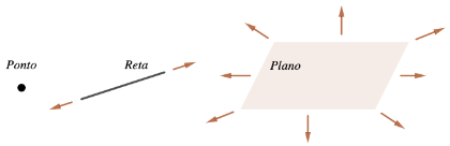
\includegraphics[keepaspectratio]{capitulos/../assets/img/01-primeiras-nocoes/Untitled.png}}

}

\caption{\label{fig-ponto-reta-plano}As setas indicando que a reta e o
plano se prolongam não serão mais desenhadas daqui por diante.}

\end{figure}%

\begin{itemize}
\tightlist
\item
  Todo ponto tem posição fixa em relação aos demais! Não se move!
\end{itemize}

\begin{definition}[]\protect\hypertarget{def-variavel-pontual}{}\label{def-variavel-pontual}

Uma variável que assume o lugar de qualquer ponto de um certo
subconjunto não vazio \(\mathcal{C}\) do plano é dita uma
\textbf{variável pontual em \(\mathcal{C}\).}

\end{definition}

\begin{tcolorbox}[enhanced jigsaw, arc=.35mm, bottomrule=.15mm, bottomtitle=1mm, breakable, colback=white, colbacktitle=quarto-callout-warning-color!10!white, colframe=quarto-callout-warning-color-frame, coltitle=black, left=2mm, leftrule=.75mm, opacityback=0, opacitybacktitle=0.6, rightrule=.15mm, title=\textcolor{quarto-callout-warning-color}{\faExclamationTriangle}\hspace{0.5em}{Aviso \ref*{wrn-ponto-movel}: Cuidado!}, titlerule=0mm, toprule=.15mm, toptitle=1mm]

\quartocalloutwrn{wrn-ponto-movel} 

Na literatura é comum se encontrar expressões como:

\begin{itemize}
\tightlist
\item
  Seja \(P\) um ponto móvel em um conjunto \(\mathcal{C}\), ou
\item
  Seja \(P\) um ponto que se move sobre um conjunto \(\mathcal{C}\)
\end{itemize}

Nestes casos \(P\) não é um ponto no sentido estrito, mas sim uma
variável pontual.

\end{tcolorbox}

\begin{tcolorbox}[enhanced jigsaw, arc=.35mm, bottomrule=.15mm, bottomtitle=1mm, breakable, colback=white, colbacktitle=quarto-callout-caution-color!10!white, colframe=quarto-callout-caution-color-frame, coltitle=black, left=2mm, leftrule=.75mm, opacityback=0, opacitybacktitle=0.6, rightrule=.15mm, title=\textcolor{quarto-callout-caution-color}{\faFire}\hspace{0.5em}{Cuidado!}, titlerule=0mm, toprule=.15mm, toptitle=1mm]

Na literatura é comum se encontrar expressões como:

\begin{itemize}
\tightlist
\item
  Seja \(P\) um ponto móvel em um conjunto \(\mathcal{C}\), ou
\item
  Seja \(P\) um ponto que se move sobre um conjunto \(\mathcal{C}\)
\end{itemize}

Nestes casos \(P\) não é um ponto no sentido estrito, mas sim uma
variável pontual.

\end{tcolorbox}

\textbf{\emph{Acrescentar aqui?}}

\begin{itemize}
\tightlist
\item
  semirretas!
\item
  segmentos aqui ?
\end{itemize}

\section{Posições Relativas Entre
Retas}\label{posiuxe7uxf5es-relativas-entre-retas}

\subsection{Definição}\label{definiuxe7uxe3o}

Duas retas \(r\) e \(s\) no plano podem ter três tipos de
\textbf{posições relativas} entre elas. Elas podem ser:

\begin{itemize}
\tightlist
\item
  \textbf{Coincidentes}: quando são iguais, isto é, \(r=s;\)
\item
  \textbf{Paralelas}: quando não se intersectam, isto é,
  \(r\cap s=\varnothing.\) Neste caso, denotamos \(r\parallel s;\)
\item
  \textbf{Concorrentes}: quando se intersectam em um ponto, isto é,
  \(r\cap s=\{P\}.\)
\end{itemize}

\bookmarksetup{startatroot}

\chapter{Distância}\label{distuxe2ncia}

\textbf{Começar com ideia intuitiva ``usando fita métrica''}

\subsection{Notação}\label{notauxe7uxe3o}

Fixada uma unidade de comprimento, a \textbf{distância entre os pontos}
\(A\) e \(B\) será denotada por \(d(A,B)\). Em geral a unidade de medida
não será mencionada, mas fica subentendido que uma unidade foi
escolhida.

\subsection{Proposição}\label{proposiuxe7uxe3o}

Valem as seguintes propriedades:

\begin{enumerate}
\def\labelenumi{\arabic{enumi}.}
\tightlist
\item
  A distância nunca é negativa. \[ d(A,B)\ge0; \]
\item
  A distância zero quando os pontos são iguais e apenas neste caso.
  \[ d(A,B)=0\Leftrightarrow A=B;\]
\item
  Medir a distância entre \(A\) e \(B\) é o mesmo que medir a distância
  entre \(B\) e \(A\). \[d(A,B)=d(B,A);\]
\item
  \(d(A,B)+d(B,C)\ge d(A,C)\);
\item
  \(d(A,B)+d(B,C)=d(A,C)\Leftrightarrow\) \(A\), \(B\) e \(C\) são
  colineares e \(B\) está entre \(A\) e \(C\).
\end{enumerate}

A propriedade 4 acima é conhecida como \textbf{desigualdade triangular}
e a propriedade 5 é um caso particular dela. Tais propriedades expressam
geometricamente que o caminho mais curto de um ponto a outro é em linha
reta.

\textbf{Exemplo}

Mova os pontos no applet abaixo e perceba que temos três desigualdades
triangulares em um mesmo triângulo.~ Coloque um dos pontos sobre o lado
oposto e observe que a propriedade 5 só vale em um dos três casos.

\bookmarksetup{startatroot}

\chapter{Segmentos}\label{segmentos}

Introduzir rapidamente e exemplificar com figura, a noção primitiva de
um ponto \textbf{estar entre} dois pontos.

\begin{definition}[]\protect\hypertarget{def-segmento}{}\label{def-segmento}

Dados dois pontos distintos \(A\)~e \(B\), sabemos que existe uma única
reta \(r\) que passa por eles. Chamamos de \textbf{segmento de reta}
\(AB\), ou simplesmente, \textbf{segmento} \(AB\) ao conjunto formado
pelos pontos \(A\) e \(B\) e pelos pontos da reta \(r\) que estão entre
\(A\) e \(B\).

Neste contexto, a reta \(r\) é chamada de \textbf{reta suporte} do
segmento \(AB\) e os pontos \(A\) e \(B\) são chamados de
\textbf{extremos do segmento} \(AB\).

\end{definition}

Note que se um ponto \(P\) está entre \(A\) e \(B\), seque ele também
está entre \(B\) e \(A\), portanto vale que \(AB=BA\).

\begin{figure}

\centering{

\pandocbounded{
\includegraphics[keepaspectratio]{capitulos/../assets/img/02-segmentos/Untitled.png}}

}

\caption{\label{fig-segmentos}}

\end{figure}%

\begin{definition}[]\protect\hypertarget{def-comprimento-segmento}{}\label{def-comprimento-segmento}

O \textbf{comprimento} ou o \textbf{tamanho} de um segmento é a
distância entre seus extremos, ou seja, o comprimento do segmento \(AB\)
é~ \(d\left(A,B\right)\).

\end{definition}

Na definição abaixo apresentamos algumas relações importantes entre dois
segmentos.

\begin{definition}[]\protect\hypertarget{def-relacoes-segmentos}{}\label{def-relacoes-segmentos}

Dois segmentos \(AB\) e \(CD\) são ditos:

\begin{itemize}
\tightlist
\item
  \textbf{Congruentes:} Se eles tem mesmo comprimento, isto é
  \(d\left(A,B\right)=d\left(C,D\right)\).
\item
  \textbf{Paralelos} ou com \textbf{mesma direção}: Se suas retas
  suporte são paralelas ou a mesma. Neste caso denotamos
  \(AB\parallel CD\).
\item
  \textbf{Perpendiculares} ou \textbf{ortogonais}:~ Se suas respectivas
  retas suporte forem perpendiculares. Neste caso denotamos~
  \(AB\perp CD\).
\end{itemize}

\end{definition}

\begin{figure}

\centering{

\pandocbounded{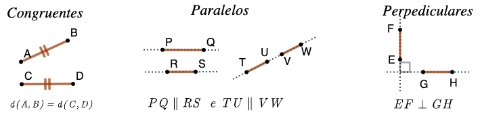
\includegraphics[keepaspectratio]{capitulos/../assets/img/02-segmentos/Untitled1.png}}

}

\caption{\label{fig-segmentos-posicao-relativa}A figura representa as
três relações entre segmentos descritas acima.}

\end{figure}%

Chamamos de segmento \textbf{degenerado} \(AA\) ao conjunto formado
apenas pelo ponto \(A\).

\begin{figure}

\centering{

\pandocbounded{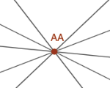
\includegraphics[keepaspectratio]{capitulos/../assets/img/02-segmentos/Untitled2.png}}

}

\caption{\label{fig-segmento-degenerado}O segmento degenerado \(AA\)
está contido em infinitas retas.}

\end{figure}%

Note que ao contrário do que ocorre com os segmentos ``não degenerados''
definidos acima, que estão contidos em uma única reta, os segmentos
degenerados estão contidos em infinitas retas.

\begin{exrr}

\caption{\label{exrr-coprimento-segmento-deg}}

\centering{

O comprimento de um segmento não degenerado pode ser~zero?

}

\end{exrr}%

\begin{tcolorbox}[enhanced jigsaw, arc=.35mm, bottomrule=.15mm, bottomtitle=1mm, breakable, colback=white, colbacktitle=quarto-callout-note-color!10!white, colframe=quarto-callout-note-color-frame, coltitle=black, left=2mm, leftrule=.75mm, opacityback=0, opacitybacktitle=0.6, rightrule=.15mm, title=\textcolor{quarto-callout-note-color}{\faInfo}\hspace{0.5em}{Resolução}, titlerule=0mm, toprule=.15mm, toptitle=1mm]

Não. Pois se \(AB\) é um segmento não degenerado então \(A\neq B\), e
portanto \(d\left(A,B\right)>0\), o que significa que o comprimento de
\(AB\) não é zero!

\end{tcolorbox}

\bookmarksetup{startatroot}

\chapter{Segmentos Orientados}\label{segmentos-orientados}

Lembremos que dada uma reta r que passa pelos pontos A e B, definimos o
\textbf{segmento de reta AB} como o conjunto formado pelos pontos \(A\)
e \(B\) e pelos pontos na reta r que estão entre \(A\) e \(B\). Agora
vamos introduzir a noção de \textbf{segmento orientado}. ****

\begin{definition}[]\protect\hypertarget{def-segmento-orientado}{}\label{def-segmento-orientado}

Um \textbf{segmento orientado} é um segmento não degenerado acrescido de
um sentido de percurso. Mais precisamente, o segmento orientado \(AB\) é
dado pelo segmento \(AB\), onde \(A\) é chamado de \textbf{ponto
inicial} e \(B\) é chamado de \textbf{ponto final}, dando a indicação de
que o sentido de percurso é~do ponto \(A\) para o ponto \(B\).

\end{definition}

Em segmentos orientados o ponto final é representado pela ponta da seta
como mostra a figura abaixo.

Seguido o raciocínio acima, o segmento orientado \(BA\) tem ponto
inicial \(B\) e ponto final \(A\) , logo o sentido de percurso é de
\(B\) para \(A\). Portanto, para segmentos orientados, \(AB \neq BA\) ,
ao contrário do que ocorre com segmentos \emph{``não orientados''},~
onde \(AB = BA\).~

Precisamos definir agora a noção de sentido entre segmentos orientados.

\begin{definition}[]\protect\hypertarget{def-sentido-semento}{}\label{def-sentido-semento}

Intuitivamente, os segmentos orientados \(AB\) e \(CD\) tem o
\textbf{mesmo sentido} se ambos são paralelos e apontam para o
``\emph{mesmo lado}''.

Note que se os segmentos orientados não tiverem mesma direção, ou seja,~
não forem paralelos, então seus sentidos são automaticamente
\textbf{diferentes}.

Nos casos em que os segmentos orientados são paralelos mas de sentidos
diferentes, também dizemos que eles tem \textbf{sentidos opostos}.

\end{definition}

Vejamos uma outra forma de definir segmentos orientados com mesmo
sentido que também aparecem em alguns livros:

\begin{definition}[]\protect\hypertarget{def-sentido-semento-formal}{}\label{def-sentido-semento-formal}

Dois segmentos orientados \(AB\) e \(CD\) tem o \textbf{mesmo sentido}
se eles são paralelos e vale um dos casos:

\textbf{Caso 1:} Se \(AB\) e \(CD\) não tem mesma reta suporte: O
segmento \(AC\) (\emph{obtido ligando o ponto inicial com ponto
inicial})~ e o segmento \(BD\) (\emph{obtido ligando ponto final com
ponto final}) não se intersectam, isto é, \(AC \cap BD = \emptyset\).

\textbf{Caso 2:}~ Se \(AB\) e \(CD\) tem mesma reta suporte \(r\):

Vamos usar um artificio para aplicar o caso 1. Tome uma reta \(s\)
paralela à reta \(r\) e sobre \(s\) considere um segmento \(A'B'\) que
tenha mesmo sentido que \(AB\) de acordo com o caso 1.~ Neste caso,
\(AB\) e \(CD\) terão o mesmo sentido se~\(CD\) também tem o mesmo
sentido de \(A’B’\) de acordo com o caso 1.

\pandocbounded{
\includegraphics[keepaspectratio]{capitulos/../assets/img/03-segmentos-orientados/Untitled.png}}

\end{definition}

\bookmarksetup{startatroot}

\chapter{Eixos}\label{eixos}

\subsection{Definição de Eixo}\label{definiuxe7uxe3o-de-eixo}

Algumas características intuitivas de tais objetos são:

\begin{definition}[]\protect\hypertarget{def-eixo}{}\label{def-eixo}

MELHORAR!!

Um \textbf{eixo} consiste de uma reta orientada \(r\) com um ponto \(O\)
fixado sobre ela, chamado de \textbf{origem}. Deste modo, \(r\) é
formada por duas semirretas com origem O, sendo que uma dessas
semirretas será dita \textbf{semieixo positivo} e será indicada com uma
seta na extremidade do desenho, e a outra semirreta (sem a seta) será
dita \textbf{semieixo negativo}.

\end{definition}

\pandocbounded{
\includegraphics[keepaspectratio]{capitulos/../assets/img/04-eixos/Untitled.png}}

Podemos associar cada ponto de um eixo com um número real da seguinte
forma:

\begin{itemize}
\tightlist
\item
  A origem \(O\) sempre corresponde ao número zero;
\item
  Se \(P\) é um ponto sobre o semieixo positivo~então \(P\) corresponde
  ao número \(p=d(P,O)\), onde \(d(P,O)\) é a distância do ponto \(P\)
  até a origem \(O\).
\item
  Se \(P\) é um ponto sobre o semieixo negativo então \(P\) corresponde
  ao número \(p=-d(P,O)\).
\item
  Se \(P\) é um ponto do eixo, então o número \(p\) obtido pelo processo
  acima é dito \textbf{coordenada} de \(P\).
\end{itemize}

\subsection{Proposição}\label{proposiuxe7uxe3o-1}

Se \(P\) e \(Q\) são pontos sobre um eixo com coordenadas \(p\) e \(q\),
respectivamente, então a distância entre \(P\) e \(Q\) é dada pela
fórmula \(d\left(P,Q\right)= | p-q|\).

\subsection{Definição de Ponto
Médio}\label{definiuxe7uxe3o-de-ponto-muxe9dio}

O \textbf{ponto médio} de um segmento \(PQ\) é o ponto \(M\) que
pertencente ao segmento e tal que
\(d\left(P,M\right)=d\left(Q,M\right)\).

\subsection{Proposição}\label{proposiuxe7uxe3o-2}

Se \(P\) e \(Q\) são pontos sobre um eixo com coordenadas \(p\) e \(q\),
respectivamente, então o ponto médio \(M\) de \(PQ\) tem coordenada
\(m=\dfrac{p+q}{2}\).

\textbf{Exemplo}

Se \(A\) e \(B\) são pontos de um eixo, tais que \(A\) tem coordenada
\(1\) e \(B\) dista \(\frac{5}{4}\) de \(A\), então \(B\) tem
coordenada:

\begin{itemize}
\item
  \(\leftarrow\) Clique para ver a solução

  \(B\) tem coordenada \(-\frac{1}{4}\) ou~ \(\frac{9}{4}\).

  De fato, suponha que \(B\) tem coordenada \(b\).~ Pela fórmula da
  distância em eixos temos~ \(\frac{5}{4}=d(A,B)=|1-b|\), logo temos
  duas possibilidades: \(1-b=\frac{5}{4}\)~e portanto \(b=-\frac{1}{4}\)
  ou~ \(1-b=-\frac{5}{4}\) e portanto \(b=\frac{9}{4}\).
\end{itemize}

\textbf{Exemplo}

Sejam \(A\) e \(B\)~pontos de um eixo, tais que \(A\) tem coordenada
\(-1\) e o ponto médio \(M\) de \(AB\) tem coordenada \(\frac{1}{2}\),
então \(B\) tem coordenada:

\begin{itemize}
\item
  \(\leftarrow\) Clique para ver a solução

  \(B\) tem coordenada 2.

  De fato, suponha que \(B\) tem coordenada \(b\). Pela Proposição acima
  temos

  \(\dfrac{1}{2}=\dfrac{-1+b}{2}\).

  E resolvendo a esta equação obtemos \(b=2\).
\end{itemize}

\textbf{Exemplo}

Seja \(\alpha\) um eixo sobre uma reta \(r\)~e sejam \(A\), \(B\) e
\(C\) pontos de \(\alpha\) com coordenadas~\(1\), \(-2\) e \(3\),
respectivamente. Suponha agora que \(\beta\) é um outro eixo sobre a
mesma reta \(r\) e com mesma unidade de medida de \(\alpha\), de modo
que a origem é o ponto \(A\) e que \(B\) tem coordenada positiva. Qual é
a coordenada de \(C\) no eixo \(\beta?\)

Dica: Faça um esboço.

\begin{itemize}
\item
  \(\leftarrow\) Click para ver a solução

  A coordenada de \(C\) no eixo \(\beta\) é \(-2\).

  De acordo com as coordenadas de \(\alpha\), o ponto \(A\) está entre
  \(B\) e \(C\).~ Como o ponto \(B\) tem coordenada negativa no eixo
  \(\alpha\) e coordenada positiva no eixo \(\beta\) os dois eixos tem
  setas em sentidos opostos (veja a figura abaixo). No eixo \(\alpha\)
  temos temos \(d(A,C)=|1-3|=2\).~Esta distância não muda no eixo
  \(\beta\), porém neste eixo \(C\) está no semieixo negativo e \(A\) é
  a origem, portanto a coordenada de \(C\) em \(\beta\) tem sinal
  negativo, isto é \(-d(A,C)=-2\).

  \pandocbounded{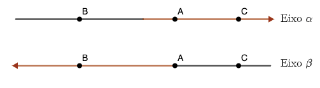
\includegraphics[keepaspectratio]{capitulos/../assets/img/04-eixos/Untitled-1.png}}
\end{itemize}

\bookmarksetup{startatroot}

\chapter{Coordenadas no plano}\label{coordenadas-no-plano}

Na seção anterior vimos, através da noção de eixo, que cada ponto de uma
reta pode ser representado por um número. Agora veremos um método para
representar cada ponto do plano através de números, mas neste caso, cada
ponto será representado por um par ordenado de números.

\begin{definition}[]\protect\hypertarget{def-sistema-eixos-ortogonais}{}\label{def-sistema-eixos-ortogonais}

Um \textbf{sistema de coordenadas cartesianas} ou um \textbf{sistema de
eixos ortogonais} \(OXY\) no plano consiste em um par de eixos com mesma
origem, \(OX\) e \(OY\) que se interceptam perpendicularmente na origem
\(O\). Assumiremos sempre que os dois eixos possuem coordenadas dadas na
mesma unidade de medida.

\end{definition}

Fixado um sistema de coordenadas \(OXY\), podemos associar cada ponto
\(P\) do plano com um único par ordenado de números reais
\(\left(x,y\right)\in\mathbb{R}^2\), chamados de \textbf{coordenadas} de
\(P\), da seguinte forma:

\begin{itemize}
\tightlist
\item
  Tome a reta \(p_X\) que é perpendicular ao eixo \(OX\) e passa pelo
  ponto \(P\)~ e tome \(X=OX\cap p_X\).
\item
  Tome a reta \(p_Y\) que é perpendicular ao eixo \(OY\) e passa pelo
  ponto P~ e tome \(Y=OY\cap p_Y\).
\item
  As coordenadas de \(P\) são dadas pelo par \(\left(x,y\right )\), onde
  \(x\) é a coordenada de \(X\) no eixo \(OX\) e \(y\) é a coordenada de
  \(Y\) no eixo \(OY\). Neste caso escrevemos \(P=\left ( x,y\right )\).
\end{itemize}

Veja a ilustração:

Usualmente chamamos o eixo \(OX\) de eixo das \textbf{abcissas} e o eixo
\(OY\) de eixo das \textbf{ordenadas}. Além disso, a menos que seja dito
o contrário, o eixo \(OX\) é o eixo horizontal e o eixo \(OY\) é o eixo
vertical.

Fixado um sistema de coordenadas ortogonais OXY, o plano é decomposto
nos eixos OX e OY e em quatro quadrantes definidos como segue:

\begin{itemize}
\tightlist
\item
  \(1^o\) quadrante =
  \(\left\{(x,y)\in\mathbb{R}^2|\,\,\, x>0,y>0\right\}\)
\item
  \(2^o\) quadrante =
  \(\left\{(x,y)\in\mathbb{R}^2|\,\,\, x<0,y>0\right\}\)
\item
  \(3^o\) quadrante =
  \(\left\{(x,y)\in\mathbb{R}^2|\,\,\, x<0,y<0\right\}\)
\item
  \(4^o\) quadrante =
  \(\left\{(x,y)\in\mathbb{R}^2|\,\,\, x>0,y<0\right\}\)
\end{itemize}

Note que os eixos não fazem parte dos quadrantes.

\pandocbounded{
\includegraphics[keepaspectratio]{capitulos/../assets/img/05-coordenadas-plano/Untitled.png}}

\begin{proposition}[]\protect\hypertarget{prp-formula-distancia}{}\label{prp-formula-distancia}

A distância entre os pontos \(P\) e \(Q\) é dada por
\[ d\left(P,Q\right)=\sqrt{\left(x_P-x_Q\right)^2+\left(y_P-y_Q\right)^2}
\]

\end{proposition}

\begin{example}[]\protect\hypertarget{exm-distancia1}{}\label{exm-distancia1}

Determine a distância do ponto \(A=(1,-1)\) até o ponto \(B=(-2,1)\).

\begin{itemize}
\tightlist
\item
  \(\leftarrow\) Click para ver a solução
\item
  \(d(A,B)=\sqrt{(1-(-2))^2+(-1-1)^2}=\sqrt{3^2+2^2}=\sqrt{13}\)
\end{itemize}

\end{example}

\begin{example}[]\protect\hypertarget{exm-distancia2}{}\label{exm-distancia2}

Determine os pontos sobre o eixo \(OX\) que distam \(\sqrt{2}\) do ponto
\(A=(1,1)\).

\begin{itemize}
\tightlist
\item
  \(\leftarrow\) Click para ver a solução
\end{itemize}

Se \(P\in OX\) temos \(P=(x,0)\). Portanto

\(\sqrt{2}=d(P,A)=\sqrt{(x-1)^2+(0-1)^2}\Rightarrow2=(x-1)^2+1\).

Resolvendo a última equação obtemos \(x=0\) ou \(x=2\). Assim temos duas
soluções para o problema: \[ P=(0,0) \text{ ou } P=(2,0). \]

\end{example}

\begin{proposition}[]\protect\hypertarget{prp-formula-ponto-medio}{}\label{prp-formula-ponto-medio}

O ponto médio \(M\) do segmento \(PQ\) tem coordenadas dadas por
\[ M=\left(\frac{x_P+x_Q}{2},\frac{y_P+y_Q}{2}\right)
\]

\end{proposition}

\begin{example}[]\protect\hypertarget{exm-ponto-medio1}{}\label{exm-ponto-medio1}

Se \(A=\left(3,-1\right)\) e \(M=\left(-1,1\right)\) é o ponto médio de
\(AB\), determine o ponto \(B\).

\begin{itemize}
\tightlist
\item
  \(\leftarrow\) Click para ver a solução
\end{itemize}

Como \(M=(-1,1)\) é ponto médio de \(A=(3,-1)\) e \(B=(x_B,y_B)\), de
acordo com a Proposição 2, temos que

\((-1,1)=\left(\dfrac{3+x_B}{2},\dfrac{-1+y_B}{2}\right)\), donde~
\(-1=\dfrac{3+x_B}{2}\) e \(1=\dfrac{-1+y_B}{2}\). Resolvendo as duas
últimas equações obtemos \(x_B=-5\) e \(y_B=3\), logo \(B=(-5,3)\).

\end{example}

\bookmarksetup{startatroot}

\chapter{Círculos}\label{cuxedrculos}

Dados um ponto \(A=\left(x_0,y_0\right)\) e um número real \(r>0\), o
\textbf{círculo de centro \(A\) e raio \(r\)} é o conjunto formado por
todos os pontos \(P\) que distam \(r\) do ponto \(A\), ou seja, o
conjunto formado pelos pontos \(P\) que satisfazem a equação
\(d\left(P,A\right)=r\).

Logo, o círculo de~ centro \(A=\left(x_0,y_0\right)\) e raio \(r\) é~
formado exatamente pelos pontos \(P=\left(x,y\right)\) que satisfazem a
equação

\[
(x-x_0)^2+(y-y_0)^2=r^2.
\]

Isso pode ser visualizado no applet a seguir.

\href{geogebra/h6vdnv3c}{Você pode mover o centro \(A\) e alterar o raio
\(r\).}

Você pode mover o centro \(A\) e alterar o raio \(r\).

\textbf{Exemplo}

Verifique se a equação representa um círculo e, em caso afirmativo,
determine o centro e o raio:

\begin{enumerate}
\def\labelenumi{\arabic{enumi}.}
\tightlist
\item
  \(x^2+y^2-2x+4y+2=0\)
\item
  \(x^2+y^2-4x+6y+13=0\)
\item
  \(x^2+y^2+3x-5y+9=0\)
\end{enumerate}

\begin{itemize}
\item
  \(\leftarrow\) Clique para ver a solução

  Para as equações descreverem círculos deve ser possível reescrevê-las
  na forma

  \((x-x_0)^2+(y-y_0)^2=r^2\). O processo usado para isso se chama
  completamento de quadrados e nele usamos o produto notável

  \[
     (u \pm a)^2 = u^2 \pm 2a u +a^2.
    \]

  \begin{enumerate}
  \def\labelenumi{\arabic{enumi}.}
  \item
    Para saber se a equação representa um círculo, vamos completar
    quadrados, usando o produto notável descrito acima:

    {\def\LTcaptype{none} % do not increment counter
    \begin{longtable}[]{@{}
      >{\raggedright\arraybackslash}p{(\linewidth - 0\tabcolsep) * \real{1.0000}}@{}}
    \toprule\noalign{}
    \begin{minipage}[b]{\linewidth}\raggedright
    \(\qquad \ x^2-2x\ \ + \ \ y^2+4y \ \ +2=0\)
    \end{minipage} \\
    \midrule\noalign{}
    \endhead
    \bottomrule\noalign{}
    \endlastfoot
    \(\Rightarrow \quad x^2-2x+{\color{blue}1-1}+y^2+4y+{\color{blue}4-4}+2=0\) \\
    \(\Rightarrow \quad{\color{green}(x^2-2x+1)}-1+{\color{blue}(y^2+4y+4)}-4+2=0\) \\
    \(\Rightarrow \quad{\color{green}(x-1)^2}-1+{\color{blue}(y+2)^2}-4+2=0\) \\
    \(\Rightarrow \quad (x-1)^2+(y+2)^2=3\). \\
    \end{longtable}
    }

    Assim temos um círculo de centro em \((1,-2)\) e raio
    \(r=\sqrt{3}\).
  \item
    Procedemos de forma análoga ao que fizemos no item 1:

    {\def\LTcaptype{none} % do not increment counter
    \begin{longtable}[]{@{}
      >{\raggedright\arraybackslash}p{(\linewidth - 0\tabcolsep) * \real{1.0000}}@{}}
    \toprule\noalign{}
    \begin{minipage}[b]{\linewidth}\raggedright
    \(\qquad \ x^2-4x\ \ + \ \ y^2+6y \ \ +13=0\)
    \end{minipage} \\
    \midrule\noalign{}
    \endhead
    \bottomrule\noalign{}
    \endlastfoot
    \(\Rightarrow \quad x^2-4x+{\color{blue}4-4}+y^2+6y+{\color{blue}9-9}+13=0\) \\
    \(\Rightarrow \quad{\color{green}(x^2-4x+4)}-4+{\color{blue}(y^2+6y+9)}-9+13=0\) \\
    \(\Rightarrow \quad{\color{green}(x-2)^2}-1+{\color{blue}(y+3)^2}-9+13=0\) \\
    \(\Rightarrow \quad (x-2)^2+(y+3)^2=0\). \\
    \end{longtable}
    }

    Note que na equação final obtemos \(r=0\), mas não existe um círculo
    de raio zero. Na verdade esta equação representa o ponto \((2,3)\),
    pois este é o único ponto que satisfaz a equação.
  \item
    {\def\LTcaptype{none} % do not increment counter
    \begin{longtable}[]{@{}
      >{\raggedright\arraybackslash}p{(\linewidth - 0\tabcolsep) * \real{1.0000}}@{}}
    \toprule\noalign{}
    \begin{minipage}[b]{\linewidth}\raggedright
    \(\qquad \ x^2+3x \ \ + \ \ y^2-5y+9=0\)
    \end{minipage} \\
    \midrule\noalign{}
    \endhead
    \bottomrule\noalign{}
    \endlastfoot
    \(\Rightarrow \quad x^2+3x+{\color{blue}\frac{9}{4}-\frac{9}{4}}+y^2-5y+{\color{blue}\frac{25}{4}-\frac{25}{4}}+9=0\) \\
    \(\Rightarrow \quad{\color{green}(x^2+3x+\frac{9}{4})}-\frac{9}{4}+{\color{blue}(y^2-5y+\frac{25}{4})}-\frac{25}{4}+9=0\) \\
    \(\Rightarrow \quad {\color{green}(x+\frac{3}{2})^2}-\frac{9}{4}+{\color{blue}(y-\frac{5}{2})^2}-\frac{25}{4}+9=0\) \\
    \(\Rightarrow \quad (x+\frac{3}{2})^2+ (y-\frac{5}{2})^2=-\frac{1}{2}\). \\
    \end{longtable}
    }

    A equação não determina um círculo. Note que a equação é
    ``absurda'', pois o lado direito não é negativo e o lado esquerdo é
    negativo! Sempre que temos uma equação absurda, ela representa o
    conjunto vazio, pois nenhum ponto pode satisfaze-la.
  \end{enumerate}
\end{itemize}

\bookmarksetup{startatroot}

\chapter{Vetores}\label{vetores}

Primeiro~ introduziremos o conceito de vetor geometricamente e, em
seguida, trataremos do conceito via coordenadas.

\subsection{Definição de Vetor}\label{definiuxe7uxe3o-de-vetor}

Um \textbf{vetor não nulo} é um objeto representado por um segmento
orientado (lembre que só consideramos segmentos orientados não
degenerados, logo \(A\neq B\)), de modo que um outro segmento orientado
\(CD\) (\(C\neq D\) ) representa o mesmo vetor se ambos os segmentos
orientados tiverem:

\begin{itemize}
\tightlist
\item
  mesmo comprimento;
\item
  mesma direção;
\item
  mesmo sentido.
\end{itemize}

Na situação acima, o vetor \(\vec{v}\) também pode ser denotado por
\(\overrightarrow{AB}\) ou por \(\overrightarrow{CD}\).

Destacamos que um vetor é representado por um segmento orientado,
contudo, o vetor não é o próprio segmento orientado. O vetor pode ser
representado por qualquer segmento orientado que possua o mesmo
comprimento, direção e sentido. É por isso que comumente falamos sobre o
movimento do vetor, no entanto, é importante lembrar que estamos, na
verdade, nos referindo a a ``trocar o representante do vetor''.

\textbf{Exemplo}

Na seguinte figura interativa mova os vetores com o mouse para
determinar quais os segmentos orientados formados pelos pontos abaixo os
representam.

\subsection{Definição de Vetor
Nulo}\label{definiuxe7uxe3o-de-vetor-nulo}

O \textbf{vetor nulo} é um vetor especial que é representado por
qualquer segmento degenerado \(AA\) , onde \(A\) é um ponto qualquer, e
é denotado por \(\vec{0}\).

Observe que só existe um vetor nulo e que, embora ele possa ser
representado por qualquer ponto ele não deve ser confundido com algum
ponto específico.

\pandocbounded{
\includegraphics[keepaspectratio]{capitulos/../assets/img/07-vetores/Untitled.png}}

\subsection{Definição}\label{definiuxe7uxe3o-1}

Dois vetores são ditos respectivamente \textbf{paralelos},
\textbf{perpendiculares}, \textbf{de mesmo sentido} ou \textbf{de
sentidos opostos} se quaisquer de seus representantes forem
respectivamente paralelos, perpendiculares, de mesmo sentido ou de
sentidos opostos.

\subsection{Definição módulo de um
vetor}\label{definiuxe7uxe3o-muxf3dulo-de-um-vetor}

O \textbf{módulo}, \textbf{comprimento} ou \textbf{norma} de um vetor
\(\vec{v}\), denotado por \(\|\vec{v}\|\), é o comprimento de segmento
qualquer segmento orientado que representa \(\vec{v}\), ou seja, se
\(\vec{v} = \vec{AB}\) então \(\| \vec{AB}\| = d(A,B)\).

Chamamos de \textbf{vetor unitário} a qualquer vetor de comprimento
\(1\).

\textbf{Obs:} O vetor nulo é o único vetor que:

\begin{itemize}
\tightlist
\item
  tem comprimento 0 , ou seja, vale:
  \(\|\vec{v}\|=0 \Leftrightarrow \vec{v}=\vec{0}\);
\item
  não tem direção;
\item
  não tem sentido.
\end{itemize}

\bookmarksetup{startatroot}

\chapter{Produto entre Número e
Vetor}\label{produto-entre-nuxfamero-e-vetor}

\subsection{Definição}\label{definiuxe7uxe3o-2}

Dados um número \(a \in \mathbb{R}\) e um vetor \(\vec{v}=(x,y)\),
definimos o produto entre eles como o vetor~ \(a\vec{v}=(ax,ay)\), ou
seja,~ \(a(x,y)=(ax,ay)\).

\textbf{Exemplo}

O produto entre o número \(2\) e o vetor \((3,-5)\) é o vetor
\(2(3,-5)=(6,-10)\).

\subsection{Proposição}\label{proposiuxe7uxe3o-3}

Valem as seguintes propriedades.

\begin{enumerate}
\def\labelenumi{\arabic{enumi}.}
\tightlist
\item
  \(1\vec{v}=\vec{v}\);
\item
  \((ab)\vec{v}=a(b\vec{v})=b(a\vec{v})\);
\item
  Se \(\vec{v}\ne\vec{0}\) então:
  \(a\vec{v}=b\vec{v}  \Leftrightarrow a=\)b;
\item
  Se \(a\ne0\) então:
  \(a\vec{v}=a\vec{w} \Leftrightarrow \vec{v}=\vec{w}\);
\item
  \(\|a\vec{v}\|=|a|\cdot\|\vec{v}\|\).
\end{enumerate}

\subsection{Definição}\label{definiuxe7uxe3o-3}

Um vetor \(\vec{u}\)~é dito múltiplo de \(\vec{v}\)~se existe um número
\(a\) tal que \(\vec{u}=a\vec{v}\).

Note que se \(\vec{u}\) e \(\vec{v}\) dois vetores não nulos e
\(\vec{u}\) é múltiplo de \(\vec{v}\) então \(\vec{v}\) é múltiplo de
\(\vec{u}\). De fato, como \(\vec{u}\) e \(\vec{v}\) são não nulos temos
que \[
\vec{u} = a\vec{v}  
\]

Para algum \(a \in \mathbb{R}\). Porém, como \(\vec{u}\) e \(\vec{v}\)
são não nulos, devemos ter \(a\neq 0\) e, desta forma, podemos realizar
a operação \[
\vec{v}=\frac{1}{a}\vec{u}
\] mostrando assim que \(\vec{v}\) é múltiplo de \(\vec{u}\).

Nesta situação também dizemos que \(\vec{u}\) e \(\vec{v}\) são
múltiplos.

A proposição a seguir fornece a interpretação geométrica do produto
entre número e vetor.

\subsection{Proposição}\label{proposiuxe7uxe3o-4}

Dados um número \(a\in\mathbb{R}\) e um vetor \(\vec{v}\), o produto
\(a\vec{v}\)~é único~vetor tal que:

Caso 1: Se \(a=0\) ou \(\vec{v}=\vec{0}\)~então~\(a\vec{v}=\vec{0}\).

Caso 2: Se \(a\ne 0\) e \(\vec{v}\ne\vec{0}\),~então \(a\vec{v}\)~é o
único vetor que satisfaz:

comprimento: \(\|a\vec{v}\|=|a|\cdot \|\vec{v}\|\);

direção: \(a\vec{v}\) é paralelo a \(\vec{v}\) (Notação:
~\(a\vec{v}\parallel\vec{v}\));

sentido:
\(a\vec{v} \,  \begin{cases}  \text{tem o mesmo sentido de } \vec{v}, & \text{ se } a>0 \\ \text{tem sentido oposto ao de } \vec{v}, &\text{ se } a<0 \end{cases}\)

\textbf{Exemplo}

\subsection{Proposição}\label{proposiuxe7uxe3o-5}

Se \(\vec{u}\) e \(\vec{v}\) são vetores não nulos temos:

\[
\vec{u} \ \text{ e }\ \vec{v} \text{ são múltiplos } \  \Leftrightarrow \vec{u}\parallel\vec{v}.
\]

\subsection{Definição}\label{definiuxe7uxe3o-4}

Por simplicidade denotaremos~\(\text{-}\,\vec{v}=(\text{-}1)\vec{v}\). O
vetor \(\text{-}\,\vec{v}\) chamado de vetor \textbf{simétrico} ou
\textbf{oposto} de \(\vec{v}\).

Note que \(\vec{v}\) e \(\text{-}\,\vec{v}\) tem mesmo comprimento e
mesma direção, mas sentidos opostos (verifique na figura iterativa
acima).

\bookmarksetup{startatroot}

\chapter{Soma e Subtração de
Vetores}\label{soma-e-subtrauxe7uxe3o-de-vetores}

\subsection{Definição}\label{definiuxe7uxe3o-5}

Se \(\vec{u}=(a_1,a_2)\) e \(\vec{v}=(b_1,b_2)\), a soma de \(\vec{u}\)
e \(\vec{v}\) e a subtração de \(\vec{u}\) por \(\vec{v}\) são os
vetores dados, respectivamente, por

\[
 \vec{u}+\vec{v}=(a_1+b_1,a_2+b_2)    \quad \text{ e } \quad  \vec{u}-\vec{v}=(a_1-b_1,a_2-b_2).
\]

\textbf{Exemplo}

Se \(\vec{u}=(2,-1)\) e \(\vec{v}=(4,3)\) então:

\[
\vec{u}+\vec{v}=(6,2), \ \vec{u}-\vec{v}=(-2,-4)  \quad \text{e} \quad   \vec{v}-\vec{u}=(2,4).
\]

\subsection{Proposição}\label{proposiuxe7uxe3o-6}

Sejam \(\vec{u}\) e \(\vec{v}\) vetores e \(a,b\in\mathbb{R}\). Valem as
seguintes propriedades:

\begin{enumerate}
\def\labelenumi{\arabic{enumi}.}
\tightlist
\item
  \(\vec{u}+\vec{0}=\vec{u}\);
\item
  \(\vec{u}+(-\vec{u})=\vec{0}\);
\item
  \(\vec{u}+(-\vec{v})=\vec{u}-\vec{v}\);
\item
  \(\vec{u}+\vec{v}=\vec{v}+\vec{u}\);
\item
  \(\vec{u}\pm(\vec{v}\pm\vec{w})=(\vec{u}\pm\vec{v})\pm\vec{w}\);
\item
  \((a\pm b)\vec{v}=a\vec{v}\pm b\vec{v}\);
\item
  \(a(\vec{v}\pm\vec{u})=a\vec{v}\pm a\vec{u};\)
\item
  \(\lVert \vec{u} + \vec{v} \rVert \leq \lVert \vec{u} \rVert + \lVert \vec{v} \rVert.\)
  \emph{Desigualdade Triangular para Vetores.}
\end{enumerate}

\subsection{Interpretação Geométrica da Soma e Subtração de
Vetores}\label{interpretauxe7uxe3o-geomuxe9trica-da-soma-e-subtrauxe7uxe3o-de-vetores}

Dados vetores \(\vec{u}\) e \(\vec{v}\), podemos representar
\(\vec{u}+\vec{v}\) e \(\vec{u}-\vec{v}\) geometricamente como segue.

Para a soma, escolhemos um representante qualquer para \(\vec{u}\),
digamos \(\vec{u}=\vec{AB}\), e para o vetor \(\vec{v}\) tomamos o
representante com ponto inicial em \(B\), obtendo \(\vec{v}=\vec{BC}\)
(o ponto inicial do representante do segundo vetor é o ponto final do
representante do primeiro vetor). A soma dos vetores é dada por

\[
 \vec{u}+\vec{v}=\vec{AB}+\vec{BC}=\vec{AC}.
\]

Para obter geometricamente subtração de \(\vec{u}\) por \(\vec{v}\), de
acordo com a propriedade \(\vec{u}-\vec{v}=\vec{u}+(-\vec{v})\), basta
aplicar a regra geométrica da soma aos vetores \(\vec{u}\) e
\(-\vec{v}\).

\textbf{Exemplo}

Note no exemplo interativo acima que:

• se \(\vec{u}\) e \(\vec{v}\) não forem paralelos, então
\(\vec{u},\vec{v}\) e \(\vec{u}\pm\vec{v}\) podem ser dispostos sobre os
lados de um triângulo.

• se \(\vec{u}\) e \(\vec{v}\) forem paralelos, então
\(\vec{u},\vec{v}\) e \(\vec{u}\pm\vec{v}\) podem ser dispostos sobre
uma mesma reta.

\bookmarksetup{startatroot}

\chapter{Combinação Linear}\label{combinauxe7uxe3o-linear}

\subsection{Definição}\label{definiuxe7uxe3o-6}

Uma \textbf{combinação linear} de vetores \(\vec{v}_1, \dots,\vec{v}_n\)
é qualquer vetor \(\vec{m}\) da forma

\[
a_1\vec{v}_1 +  \cdots + a_n\vec{v}_n, 
\] onde \(a_1, \dots, a_n\) são números reais.

\textbf{Exemplo}

No exemplo interativo abaixo, abordaremos o caso \(n=3\), ou seja,
veremos algumas combinações lineares de três vetores
\(\vec{v}_1, \ \vec{v}_2\) e \(\vec{v}_3\).

\textbf{Exemplo}

Quais vetores são obtidos como combinação linear de um único vetor
\(\vec{v}\) ?

\begin{itemize}
\tightlist
\item
  \(\leftarrow\) Click para ver a solução
\end{itemize}

Qualquer vetor \(\vec{m}\) que for múltiplo de \(\vec{v}\), ou seja,
\(\vec{m} = a \vec{v}\), com \(a \in \mathbb{R}\).

\subsection{Proposição}\label{proposiuxe7uxe3o-7}

Fixados dois vetores não paralelos \(\vec{u}\) e \(\vec{v}\), qualquer
outro vetor do plano \(\vec{w}\) se escreve de maneira única como
combinação linear de \(\vec{u}\) e \(\vec{v}\), ou seja, para cada
\(\vec{w}\) existe um único \(a\in \mathbb{R}\) e existe um único
\(b\in \mathbb{R}\) tais que \(\vec{w}=a\vec{u}+b\vec{v}.\)

\textbf{Exemplo}

Determine o vetor \(\vec{w}=(3,-5)\) como combinação linear de
\(\vec{u}=(1,-1)\) e \(\vec{v}=(2,3)\).

\begin{itemize}
\item
  \(\leftarrow\) Click para ver a solução

  Devemos encontrar \(a\) e \(b\) tais que
  \(\vec{w}=a\vec{u}+b\vec{v}.\) Substituindo as coordenadas dos vetores
  na expressão anterior temos \((3,-5)=a(1,-1)+b(2,3)=(a+2b,-a+3b)\), e
  portanto

  \[
    \left\{ \begin{array}{l} a +2b = 3 \\ -a + 3b = -5. \end{array} \right.
    \]

  Resolvendo o sistema obtemos \(a=\frac{19}{5}\) e \(b=-\frac{2}{5}\).
  Logo temos a combinação linear

  \[
    \vec{w}=\frac{19}{5}\vec{u}-\frac{2}{5}\vec{v}
    \]
\end{itemize}

\textbf{Exemplo}

Escreva o vetor \(\vec{p}=(1,3)\) como combinação linear dos vetores
\(\vec{u}=(1,0),\vec{v}=(0,-1)\) e \(\vec{w}=(-1,1)\) de três maneiras
distintas.

\begin{itemize}
\tightlist
\item
  \(\leftarrow\) Click para ver a solução
\end{itemize}

Existem infinitas possibilidades, de acordo com a proposição acima. Por
exemplo:

\(\vec{p}=\vec{u}-3\vec{v}\) ou \(\vec{p}=2\vec{u}-2\vec{v}+\vec{w}\) ou
\(\vec{p}=4\vec{u}+3\vec{w}\).

\textbf{Resolução:} Devemos encontrar \(a,b\) e \(c\) tais que
\(\vec{p}=a\vec{u}+b\vec{v}+c\vec{w}.\) Substituindo as coordenadas dos
vetores dados, na expressão anterior, temos \[
    (1,3)=a(1,0)+b(0,-1)+c(-1,1)=(a-c,-b+c) 
\] e portanto \[
    \left\{ \begin{array}{l}  a-c=1\\ -b+c=3. \end{array} \right.
\]

Como o sistema acima possui duas equações e três variáveis, ele tem
infinitas soluções. Por exemplo, resolvendo \(a\) e \(b\) em função de
\(c\), segue que

\[
    \vec{p} = (c+1) \vec{u} + (c-3) \vec{v} +c\vec{w} \quad \forall \ c \in \mathbb{R}.
\]

Assim, vejamos três possibilidades de combinações, fazendo \(c=0,\ c=1\)
e \(c=3\), respectivamente:

\begin{verbatim}
$$
\vec{p}=\vec{u}-3\vec{v}
$$

$$
\vec{p}=2\vec{u}-2\vec{v}+\vec{w}
$$

$$
\vec{p}=4\vec{u}+3\vec{w}
$$
\end{verbatim}

\bookmarksetup{startatroot}

\chapter{Produto Interno ou Escalar}\label{produto-interno-ou-escalar}

\subsection{Definição 1}\label{definiuxe7uxe3o-1-1}

Dados vetores \(\vec{u}=(a_1,a_2)\) e \(\vec{v}=(b_1,b_2)\), o produto
interno ou escalar entre eles é definido por \[
\left\langle\vec{u},\vec{v}\right\rangle=a_1b_1+a_2b_2.
\]

Alguns livros usam a seguinte notação para produto interno:
\(\vec{u}.\vec{v}\)

\textbf{Exemplo}

Por exemplo, se \(\vec{u}=(1,-4)\) e \(\vec{v}=(3,2)\) então 

\[
\langle \vec{u} ,\vec{v}\rangle=1\cdot3+(-4)\cdot2=-5.
\]

\subsection{Proposição 1}\label{proposiuxe7uxe3o-1-1}

Valem as seguintes propriedades:

\begin{enumerate}
\def\labelenumi{\arabic{enumi}.}
\tightlist
\item
  \(\langle \vec{u}, \vec{u} \rangle = \|\vec{u}\|^2\);
\item
  \(\left\langle\vec{u},\vec{v}\right\rangle=\left\langle\vec{v},\vec{u}\right\rangle\);
\item
  \(\left\langle
  a\vec{u},\vec{v}\right\rangle=\left\langle\vec{u},a\vec{v}\right\rangle=a\left\langle\vec{u},\vec{v}\right\rangle\);
\item
  \(\left\langle\vec{v}+\vec{w},\vec{u}\right\rangle=\left\langle\vec{v},\vec{u}\right\rangle+\left\langle\vec{w},\vec{u}\right\rangle\);
\item
  \(\left\langle\vec{u,}\vec{v}+\vec{w}\right\rangle=\left\langle\vec{u},\vec{v}\right\rangle+\left\langle\vec{u},\vec{w}\right\rangle\).
\end{enumerate}

\subsection{\texorpdfstring{\textbf{Interpretação geométrica do produto
interno.}}{Interpretação geométrica do produto interno.}}\label{interpretauxe7uxe3o-geomuxe9trica-do-produto-interno.}

O produto interno entre dois vetores está intimamente relacionado com o
comprimento dos vetores e o ângulo formado por eles, como veremos.

\subsection{Definição 2}\label{definiuxe7uxe3o-2-1}

Dados dois vetores não nulos \(\vec{u}\) e \(\vec{v}\), podemos supor
\(\vec{u}=\vec{OA}\) e \(\vec{v}=\vec{OB}\). Definimos o ângulo entre os
vetores \(\vec{u}\) e \(\vec{v}\), denotado por
\(\sphericalangle(\vec{u},\vec{v})\), como sendo a menor medida positiva
do ângulo (menor ângulo) \(A\hat{O}B\).

\subsection{Proposição 2}\label{proposiuxe7uxe3o-2-1}

O produto interno entre \(\vec{u}\) e \(\vec{v}\) satisfaz

\[
\left\langle\vec{u},\vec{v}\right\rangle=\|\vec{u}\|\:\|\vec{v}\| \cos \sphericalangle
(\vec{u},\vec{v}).
\]

A próxima proposição é consequência do resultado acima e e será muito
utilizada ao longo do curso.

\subsection{Proposição 3}\label{proposiuxe7uxe3o-3-1}

Se \(\vec{u}\) e \(\vec{v}\) são vetores não nulos, dizemos que eles são
perpendiculares ( \(\vec{u}\perp\vec{v}\) ) se, e somente se

\[
\langle\vec{u},\vec{v}\rangle=0\Leftrightarrow
\sphericalangle(\vec{u},\vec{v}) = 90^\circ.
\]

\textbf{Exemplo}

Dado um número \(a\ne0\), determine o ângulo entre o vetores
\(\vec{u}=(1,-1)\) e \(\vec{v}=(0,a)\), de acordo com o sinal de \(a\).

\begin{itemize}
\item
  \(\leftarrow\) Click para ver a solução

  \textbf{Resposta:}
  \(\sphericalangle(\vec{u},\vec{v})=135^\circ \text{ se } a>0 \quad \text{ e }  \quad \sphericalangle(\vec{u},\vec{v})=45^\circ  \text{ se } a<0\).

  \textbf{Resolução:} Pela Proposição 1 temos

  \[
     \langle\vec{u},\vec{v}\rangle=\lVert\vec{u}\rVert\lVert\vec{v}\rVert cos\sphericalangle(\vec{u},\vec{v}).
    \]

  Como \(\vec{u}\) e \(\vec{v}\) não são nulos temos
  \(\lVert\vec{u}\rVert\lVert\vec{v}\rVert\neq0\). Dividindo a equação
  acima por \(\lVert\vec{u}\rVert\lVert\vec{v}\rVert\) obtemos

  \[
    \cos\sphericalangle(\vec{u},\vec{v})=\frac{\langle\vec{u},\vec{v}\rangle}{\lVert\vec{u}\rVert\lVert\vec{v}\rVert} \quad (\ast).
    \]

  Mas note que \[
    \langle\vec{u},\vec{v}\rangle=\langle (1,-1),(0,a) \rangle=-a , \\ \lVert\vec{u}\rVert=\sqrt{1^2+(-1)^2}=\sqrt{2}\\\lVert\vec{v}\rVert=\sqrt{0^2+a^2}=|a| .
    \]

  Portanto, por \((\ast)\), temos

  \(\cos\sphericalangle\left(\vec{u},\vec{v}\right)=\frac{-a}{\sqrt{2}\mid a\mid}=\frac{-a\sqrt{2}}{\mid a\mid2}=\begin{cases}
    \frac{-\sqrt{2}}{2}\quad  se\quad a>0 \\
    \frac{\sqrt{2}}{2}\quad  se\quad a<0
    \end{cases}\) Donde segue o resultado!
\end{itemize}

\bookmarksetup{startatroot}

\chapter{Projeção Ortogonal}\label{projeuxe7uxe3o-ortogonal}

\subsection{Definição}\label{definiuxe7uxe3o-7}

Dados vetores \(\vec{u}\) e \(\vec{v}\), com \(\vec{u}\ne\vec{0}\),
definimos a projeção ortogonal de \(\vec{v}\) em \(\vec{u}\) como sendo
o vetor dado por

\[
 {Proj}_{\:\vec{u}}\: \vec{v} = \frac{\langle \vec{v},\vec{u}\rangle}{\lVert \vec{u} \rVert^2}\vec{u}.
\]

\textbf{Exemplo}

Por exemplo, se \(\vec{u}=(1,1)\) e \(\vec{v}=(2,3)\) temos \[
{Proj}_{\:\vec{u}}\:\vec{v}  =\frac{\langle (2,3), (1,1) \rangle}{\rVert(1,1)
\lVert^2}(1,1)=\frac{5}{2}(1,1)=\left(\frac{5}{2},\frac{5}{2}\right).
\]

\subsection{\texorpdfstring{\textbf{Interpretação Geométrica da Projeção
Ortogonal.}}{Interpretação Geométrica da Projeção Ortogonal.}}\label{interpretauxe7uxe3o-geomuxe9trica-da-projeuxe7uxe3o-ortogonal.}

Intuitivamente, se imaginarmos que o vetor \(\vec{u}\) é paralelo ao
``solo'' então o vetor \({ Proj}_{\:\vec{u}}{\:\vec{v}}\) corresponde a
``sombra'' que o vetor \(\vec{v}\) projeta no solo ao meio dia.

\pandocbounded{
\includegraphics[keepaspectratio]{capitulos/../assets/img/12-projecao-ortogonal/untitled.png}}

Além disso, se os vetores \(\vec{u}\) e \(\vec{v}\) não forem paralelos
nem perpendiculares, então os vetores \({ Proj}_{\:\vec{u}}{\:\vec{v}}\)
e \(\vec{v}- { Proj}_{\:\vec{u}}{\:\vec{v}}\) podem ser representados
sobre os catetos de um triângulo retângulo tendo \(\vec{v}\) sobre a
hipotenusa.

Em particular, se \(\vec{v}\neq\vec{p}= { Proj}_{\:\vec{u}}\:\vec{v}\) ,
isto é, se \(\vec{v}- { Proj}_{\:\vec{u}}\:\vec{v} \neq \vec{0}\),
observamos, na representação acima, que
\(\vec{v}- { Proj}_{\:\vec{u}}\:\vec{v} \perp \vec{u}\). Esta
propriedade está descrita no item 2 da próxima proposição.

\subsection{Proposição}\label{proposiuxe7uxe3o-8}

Nas condições da definição acima valem as seguintes propriedades.

\begin{enumerate}
\def\labelenumi{\arabic{enumi}.}
\tightlist
\item
  Se \({ Proj}_{\:\vec{u}}\:\vec{v} \neq \vec{0}\) então
  \({ Proj}_{\:\vec{u}}\:\vec{v} \parallel \vec{u}\);
\item
  Se \(\vec{v}- { Proj}_{\:\vec{u}}\:\vec{v} \neq \vec{0}\) então
  \(\vec{v}- { Proj}_{\:\vec{u}}\:\vec{v} \perp \vec{u}\);
\item
  Se \(a \neq 0\) então
  \({ Proj}_{\:a\vec{u}}\:\vec{v} = { Proj}_{\:\vec{u}}\:\vec{v}\);
\item
  \({ Proj}_{\:\vec{u}}\:a\vec{v} = a \;{ Proj}_{\:\vec{u}}\:\vec{v}\);
\item
  \({ Proj}_{\:\vec{u}}\:(\vec{v} + \vec{w}) ={ Proj}_{\:\vec{u}}\:\vec{v} + { Proj}_{\:\vec{u}}\:\vec{w}\).
\end{enumerate}

\bookmarksetup{startatroot}

\chapter{Área de triângulos e
paralelogramos}\label{uxe1rea-de-triuxe2ngulos-e-paralelogramos}

\subsection{Definição}\label{definiuxe7uxe3o-8}

Dizemos que um paralelogramo \(\mathcal{P}\) tem lados \(\vec{u}\) e
\(\vec{v}\) se um dos lados orientados de \(\mathcal{P}\) for
representante de \(\vec{u}\) e o outro lado orientado de \(\mathcal{P}\)
for representante de \(\vec{v}\).

\pandocbounded{
\includegraphics[keepaspectratio]{capitulos/../assets/img/13-area-triangulos-paralelogramos/untitled.png}}

\subsection{Proposição}\label{proposiuxe7uxe3o-9}

Se \(\vec{u}=\left(a_1,a_2\right)\) e \(\vec{v}=\left(b_1,b_2\right)\)
são os lados de um paralelogramo \(\mathcal{P}\), como na figura acima,
então a área de \(\mathcal{P}\) é dada por

\[
  Área\mathcal{P} = \left| det
\begin{pmatrix}
- \ \vec{u} \ - \\
- \ \vec{v} \ -
\end{pmatrix}  \right| =  \left| det \begin{pmatrix}
a_1 & a_2 \\
b_1 & b_2
\end{pmatrix}  \right|.
\]

\textbf{Exemplo}

Determine a área do triângulo de vértices \(A=(0,-1), \; B=(-1,2)\) e
\(C=(3,1)\).

\begin{itemize}
\item
  \(\leftarrow\) Click para ver a solução

  A área do triângulo \(ABC\) é a metade da área do paralelogramo
  correspondente aos vetores (veja figura abaixo).

  \[
    \vec{AB}=B-A=(-1,3)  \\ \vec{AC}=C-A=(3,2)
    \] portanto, de acordo com a Proposição 1 acima, sua área é dada por

  \pandocbounded{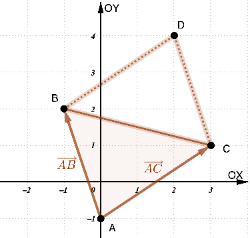
\includegraphics[keepaspectratio]{capitulos/../assets/img/13-area-triangulos-paralelogramos/material-eu2tdbpc.png}}

  \[
    Área(ABC)=\frac{1}{2} \left| det \begin{pmatrix}
    \vec{AB} \\
    \vec{AC}
    \end{pmatrix}  \right| = \frac{1}{2} \left| det \begin{pmatrix}
    -1 & 3 \\
    3 &  2
    \end{pmatrix}  \right|= \frac{1}{2} \left|   -11 \right| = \frac{11}{2}.
    \]
\end{itemize}

\bookmarksetup{startatroot}

\chapter{}\label{section-1}

Equação Paramétrica de Reta

Destacamos as seguintes propriedades:

\emph{Por dois pontos distintos passa uma única reta.}

Dadas duas retas distintas \(r\) e \(s\) temos duas possibilidades
quanto sua interseção:

\begin{enumerate}
\def\labelenumi{\arabic{enumi}.}
\tightlist
\item
  \emph{r e s não se intersectam, isto é, \(r\cap s=\varnothing\). Neste
  caso, r e \(s\) são ditas paralelas ou com mesma direção e denotamos
  \(r\parallel s\)}
\item
  \emph{r e s se intersectam em um único ponto.Neste caso, \(r\) e \(s\)
  são ditas concorrentes.}
\end{enumerate}

Duas retas concorrentes \(r\) e \(s\), formando ângulos de
\(90^{\circ}\) são ditas perpendiculares ou ortogonais e denotamos por
\(r\perp s.\)

\pandocbounded{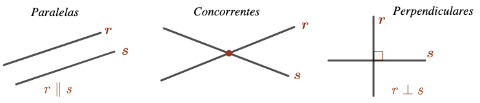
\includegraphics[keepaspectratio]{capitulos/../assets/img/14-eq-parametrica-reta/untitled-1.png}}

Definição

Dizemos que um vetor \(\vec{u}\) é um vetor diretor ou um vetor paralelo
a uma reta \(r,\) e denotamos \(\vec{u}\parallel r\) quando \(\vec{u}\)
pode ser representado sobre a reta \(r,\) ou seja, quando existem dois
pontos \(A\) e \(B\) da reta tais que \(\vec{u} = \overrightarrow{AB}.\)

\textbf{Proposição}

Fixados um ponto \(P_0\) e um vetor \(\vec{v}\ne\vec{0},\) existem
infinitas retas paralelas a \(r,\) mas existe apenas uma reta paralela a
\(\vec{v}\) que passa por \(P_0.\)

Fixados um ponto \(P_0\) e um vetor \(\vec{v}\ne\vec{0},\) considere a
única reta \(r\) tal que \(P_0\in r\) e \(\vec{v}\parallel r.\)

Um ponto \(P\) do plano pertence a reta \(r\) se, e somente se, o vetor
\(P-P_0=\vec{P_0P}\) é múltiplo de \(\vec{v}\), isto é,
\(P-P_0=t\vec{v}\), com \(t\in\mathbb{R}\). Portanto, a reta \(r\) é
dada pela equação:

\[
r: P = P_0 + t \vec{v}, \quad t \in \mathbb{R}. \quad(\ast)
\]

\textbf{Observação:} Na equação acima o ponto \(P_0\in r\) e o vetor
\(\vec{v}\parallel r\) são constantes, pois eles foram fixados a priori,
já o ponto \(P\) e o número \(t\) são variáveis, uma vez que \(P\)
percorre a reta \(r\) a medida que \(t\) percorre \(\mathbb{R}\). De
fato, \(P\) e \(t\) são variáveis dependentes uma da outra, pois para
cada \(P\in r\) existe um único \(t\in \mathbb{R}\) que satisfaz a
equação e vice versa.

Definição

Qualquer equação da forma \((\ast)\) é dita equação paramétrica de
\(r\). Neste caso, a variável \(t\) é chamada de parâmetro da equação e
o ponto \(P_0\) e o vetor \(\vec{v}\) são chamados de elementos fixos da
equação.

\textbf{Observação:} Existem infinitas equações paramétricas para uma
mesma reta. De fato, existem infinitas possibilidades de escolha os
elementos fixos e escolhas distintas fornecem equações paramétricas
distintas para a reta. Veja as Atividades e o Exemplo 2 abaixo.

Nesta atividade você pode ver a relação entre cada ponto de uma reta e
seu correspondente parâmetro de acordo com diferentes escolhas dos
elementos fixados.

Mova o ponto \(P\) para ver sua relação com o parâmetro \(t\).

Mova o ponto \(P\) para ver sua relação com o parâmetro \(t\).

Vejamos como a equação paramétrica
\(r: P = P_0 + t \vec{v}, \ t \in \mathbb{R}\) fica usando coordenadas.

Ponha \(P=(x,y)\) e suponha que os elementos fixos da equação de \(r\)
são dados em coordenadas por \(P_0=(x_0,y_0)\in r\) e
\(\vec{v}=(a,b)\parallel r\) . Substituindo na equação acima, temos:

\[
r: \: (x, y) = (x_0,y_0) + t(a, b) = (x_0 + at , y_0+ bt), \ t\in \mathbb{R}.
\]

Igualando as coordenadas podemos reescrever a equação da forma

\[
\begin{array}{llr}
r:\left\lbrace \begin{array}{l}x={\color{993300}x_0}\; + \;{\color{D2691E}a}t \\
y={\color{993300}y_0}\; + \;{\color{D2691E}b}t  \\
\end{array} \right.,  \ \ t\in\mathbb{R}. &\ \ \ (\ast \ast)\\
\begin{array}{l}
 \ \ \ \quad \uparrow \; \ \quad \uparrow  \qquad  \uparrow \\
\ \  \quad P={\color{993300}P_0}+  t{\color{D2691E}\vec{u}}
\end{array} & & 
\end{array}
\]

No applet abaixo você pode alterar os elementos fixos das retas e
verificar as suas respectivas equações paramétricas.

\url{geogebra/g8j8szyk}

\textbf{Exemplo}

Verifique se os pontos que \(A=(-2,7)\) e \(B=(7,-2)\) pertencem a reta

\[
r: \left\{
\begin{array}{l}
x = 1 + 3t \\
y = 2 - 5t
\end{array}
\right. , \ t \in \mathbb{R}.
\]

\begin{itemize}
\item
  \(\leftarrow\) Click para ver a solução.

  Para um ponto pertencer a reta \(r\) suas coordenadas devem satisfazer
  sua equação paramétrica para um \textbf{único} valor do parâmetro
  \(t \in \mathbb{R}\).

  Substituindo o ponto \(A\) na equação de \(r\) acima obtemos

  \[
    \begin{array}{lcl}
    -2 = 1 + 3t & \Rightarrow &t=-1 \\
    7 = 2 - 5t & \Rightarrow & t=-1.
    \end{array}
    \]

  Como obtemos um único valor de t segue que \(A\in r\).

  Substituindo o ponto \(B\) na equação de \(r\) segue que

  \[
    \begin{array}{lcl}
    7 = 1 + 3t &\Rightarrow & t= -2\\
    -2 = 2 - 5t &\Rightarrow & t=\frac{4}{5}
    \end{array}
    \]

  Como obtemos dois valores distintos para \(t\) temos que
  \(B \notin r\).
\end{itemize}

\textbf{Exemplo}

Determine duas equações paramétricas para cada reta abaixo.

\begin{enumerate}
\def\labelenumi{\arabic{enumi}.}
\tightlist
\item
  \(\ell\) é a reta que passa pelo ponto \(P_0=(2,1)\) e é paralela ao
  vetor \(\vec{u}=(1,-3)\);
\item
  \(m\) é a reta que passa pelos pontos \(A=(-2,-1)\) e \(B=(-1,2).\)
\end{enumerate}

\begin{itemize}
\item
  \(\leftarrow\) Click para ver a solução

  Como sabemos, existem infinitas equações paramétricas para cada reta
  as quais dependerão da escolha de seus elementos fixos.

  \begin{enumerate}
  \def\labelenumi{\arabic{enumi}.}
  \tightlist
  \item
    Para a reta \(\ell\), temos por exemplo:

    \begin{enumerate}
    \def\labelenumii{\arabic{enumii}.}
    \item
      Substituindo os elementos fixos \(P_0\) e \(\vec{u}\) nas equações
      \((\ast \ast)\) acima, obtemos

      \$\$ \ell: \left\{

      \begin{array}{l}
       x = 2 + t \\
       y = 1 - 3t
       \end{array}

      \right. , ~t \in \mathbb{R}.

      \$\$
    \item
      Tomando o parâmetro \(t=1\) na equação do item a., obtemos o ponto
      \(P_1 =(3,-2)\in \ell\) e multiplicando o vetor \(\vec{u}\) por
      \(-2\) obtemos o vetor
      \(\vec{v}= -2\vec{u}= (-2,6) \parallel \ell.\) Assim, usando os
      novos elementos fixos elementos fixos \(P_1\) e \(\vec{v}\)
      deduzimos a seguinte equação

      \$\$ \ell: \left\{

      \begin{array}{l}
       x = 3 -2s \\
       y = -2 +6s
       \end{array}

      \right. , ~s \in \mathbb{R}.

      \$\$
    \end{enumerate}
  \item
    Para a reta \(m\), temos por exemplo:

    \begin{enumerate}
    \def\labelenumii{\arabic{enumii}.}
    \item
      Tomando como elementos fixos o ponto \(A=(-2,-1) \in m\) e o vetor
      \(\overrightarrow{AB}=B-A=(1,3)\) \(\parallel m\), obtemos:

      \$\$ m: \left\{

      \begin{array}{l}
       x = -2 + \mu \\
       y = -1 +3\mu
       \end{array}

      \right. , ~\mu \in \mathbb{R}.

      \$\$
    \item
      Tomando como elementos fixos o ponto \(B=(-1,2) \in m\) e o vetor
      \(\tfrac{1}{2}\overrightarrow{BA}=(-\tfrac{1}{2},-\tfrac{3}{2}) \parallel m\),
      obtemos:

      \$\$ m: \left\{

      \begin{array}{l}
       x = -1 -\tfrac{1}{2} \nu \\
       y = 2 -\tfrac{3}{2}\nu
       \end{array}

      \right. , ~\nu \in \mathbb{R}.

      \$\$
    \end{enumerate}
  \end{enumerate}
\end{itemize}

\bookmarksetup{startatroot}

\chapter{Equação Cartesiana da
Reta}\label{equauxe7uxe3o-cartesiana-da-reta}

\subsection{Definição}\label{definiuxe7uxe3o-9}

Dizemos que um vetor \(\vec{u}\) não nulo é normal ou perpendicular a
uma reta \(r\), e denotamos \(\vec{u} \perp r\), se \(\vec{u}\) é
perpendicular ao vetor \(\overrightarrow{AB}\), quaisquer que sejam os
pontos \(A, B \in r\).

\subsection{Proposição}\label{proposiuxe7uxe3o-10}

Dados um ponto \(P_0\) e um vetor \(\vec{u} \neq \vec{0}\), existem
infinitas retas perpendiculares a \(\vec{u}\), mas existe apenas uma
reta \(r\) que é perpendicular ao vetor \(\vec{u}\) e que passa pelo
ponto \(P_0\).

Fixados um ponto \(P_0 = (x_0, y_0)\) e um vetor
\(\vec{u} = (a, b) \neq \vec{0}\), considere a única reta \(r\) tal que
\(P_0 \in r\) e \(\vec{u} \perp r\).

Um ponto \(P = (x, y) \in r\) se, e somente se, o vetor
\((x - x_0, y - y_0) = P - P_0 = \overrightarrow{P_0P}\) é perpendicular
a \(\vec{u}\), isto é,

\[
\begin{array}{lcl}\langle (x - x_0, y - y_0), (a, b) \rangle = 0 & \Leftrightarrow &  a(x - x_0) + b(y - y_0) = 0 \\           &\Leftrightarrow &  ax + by + \underbrace{(-ax_0 - by_0)}_{\text{constante}} = 0.\end{array}
\]

Deste modo, concluímos que um ponto \(P = (x, y)\) pertence à reta
\(r\), se, somente se, ele satisfaz a equação

\[
r: \: \underbrace{ax + by}_{(a,b)\perp r} + c= 0 \quad (\ast) \quad \text{ ou então } \quad r: \: \underbrace{ax + by}_{(a,b)\perp r} = c' \quad (\ast \ast), 
\]

onde \(c =-( ax_0 + by_0)\) e \(c'=  ax_0 + by_0\) são constantes.

Note que os coeficientes \(a\) e \(b\) das equações (\(\ast\)) e
(\(\ast \ast\)) são as coordenadas do vetor perpendicular a reta \(r\).

\subsection{Definição}\label{definiuxe7uxe3o-10}

Qualquer equação da forma \((\ast)\) ou \((\ast\ast)\) acima é dita
equação cartesiana da reta \(r\).

\subsection{Proposição}\label{proposiuxe7uxe3o-11}

Duas equações da forma \((\ast)\) representam a mesma reta se, e somente
se, elas diferem pela multiplicação de uma constante não nula. Dito de
outra forma:

As equações \(ax+by+c=0\) e \(a’x+b’y+c’=0\) descrevem a mesma reta se,
e somente se,

\[
   a’=\lambda a, \quad b’=\lambda b \quad\text{e}\quad  c’=\lambda c \quad \text{ para algum número real}\quad \lambda \neq 0.
\]

\textbf{Exemplo}

Determine a equação cartesiana da reta \(m\) que passa pelo ponto
\(B = (7, 11)\) e é normal ao vetor \(\vec{u} = (-3, 4)\).

\begin{itemize}
\item
  \(\leftarrow\) Click para ver a solução

  Como \((a,b)=(-3,4) \perp m\), a equação cartesiana de \(m\) tem a
  forma

  \(m: -3x+4y+c=0\). Para determinar a constante \(c\) não é necessário
  usar a formula dada em \((\ast)\), basta substituir as coordenadas de
  um ponto da reta na expressão que já temos. Usando o ponto \(B \in m\)
  segue que

  \[
    -3(7) + 4(11) + c=0 \quad  \Rightarrow \quad  c=-23.
    \]

  Logo,

  \[
     m: -3x+4y-23=0.
    \]

  \textbf{Obs.} Pela Proposição 1 também temos

  \[
     m: 3x - 4y+ 23=0 \quad \text{ ou } \quad  m: 6x - 8y+ 46=0.
    \]
\end{itemize}

\textbf{Observação}:

Lembremos que, dada uma reta r:

\[
\vec{u} = (a, b) \perp r \quad \Leftrightarrow \quad \vec{v} = (b,-a) \parallel r.
\]

\textbf{Exemplo}

Determine a equação cartesiana da reta\\
\(r: \left\lbrace
\begin{array}{l}
x = 5 - 4t \\
y = -2 + t
\end{array}
\right.,\ t \in \mathbb{R}.\)

\begin{itemize}
\item
  \(\leftarrow\) Click para ver a solução

  \textbf{Primeira resolução:} Para obter uma equação cartesiana de
  \(r\) precisamos de um ponto de \(r\) e de um vetor perpendicular a
  \(r\).

  Da equação original obtemos que \(P_0 = (5,-2) \in r\) e
  \(\vec{v}=(-4,1)\parallel r\). Pela observação acima segue que
  \(\vec{u}=(1,4) \perp r\).

  Portanto \(r:1x+4y+c=0\) e substituindo as coordenadas de \(P_0\) na
  equação obtemos \(1(5)+4(-2) + c=0 \ \Rightarrow \ c=3\). Logo

  \[
    r: x+4y+3=0.
    \]

  \textbf{Segunda resolução:} Da equação paramétrica de \(r\) temos
  \(t=y+2\) e substituindo na outra equação segue que \(x= 5 - 4(y+2)\),
  donde obtemos a mesma equação de \(r\) acima.
\end{itemize}

\textbf{Exemplo}

Determine as equações paramétricas da reta \(s \colon -7x + 2y = 8\).

\begin{itemize}
\item
  \(\leftarrow\) Click para ver a solução

  \textbf{Primeira resolução:} Para obter uma equação paramétrica de
  \(s\) precisamos de um ponto de \(s\) e de um vetor paralelo a \(s\).

  Para obtermos um ponto de \(s\), basta escolher um valor específico
  para uma das variáveis da equação original e determinar o valor da
  outra variável. Por exemplo, tomando \(x=0\) na equação acima temos
  \(-7(0) + 2y=8 \Rightarrow y=4\). Logo o ponto \((0,4) \in s\).

  Para obtermos um vetor paralelo a \(s\) note que
  \(\vec{u}=(-7,2) \perp s\) e segue observação acima que
  \(\vec{v}=(2,7)\parallel s\).

  Portanto uma equação paramétrica de \(s\) é

  \[
    s \colon \left\lbrace \begin{array}{l} x= 0 + 2t \\ y=4+7t  \end{array} \right. , \ t \in \mathbb{R},  \quad \text{ou seja,} \quad  s \colon \left\lbrace \begin{array}{l} x= 2t\\ y=4+7t  \end{array} \right., \ t \in \mathbb{R}.
    \]

  \textbf{Segunda resolução:} Consideramos uma das variáveis como
  parâmetro e obtemos a outra variável em função do parâmetro. Por
  exemplo, tomando \(x=t\) e substituindo na equação de \(s\) temos
  \(-7t + 2y=8\ \Rightarrow \ y=4 -\frac{7}{2}t\). Portanto uma equação
  paramétrica de \(s\) é

  \[
    s \colon \left\lbrace \begin{array}{l} x= t\\ y=4+\frac{7}{2}t  \end{array} \right., \ t \in \mathbb{R}.
    \]

  Em cada resolução obtivemos equações paramétricas diferentes para a
  mesma reta \(s\), mas lembre que para uma mesma reta existem infinitas
  equações paramétricas.
\end{itemize}

\bookmarksetup{startatroot}

\chapter{Interseção de Retas}\label{interseuxe7uxe3o-de-retas}

\subsection{Proposição}\label{proposiuxe7uxe3o-12}

O ponto de interseção entre retas dadas por equações é o ponto
\((x,y)\), onde \(x\) e \(y\) são soluções do sistema obtido pelas
equações das retas envolvidas.

\textbf{Exemplo}

Determine o ponto de interseção entre as retas

\[
 \ell: x-2y=0 \quad \text{ e } \quad m: \left\{ \begin{array}{l} x= 1+t \\ y =2 -t\end{array} \right. , t \in \mathbb{R}.
\]

\begin{itemize}
\item
  \(\leftarrow\) Click para ver a solução

  O sistema obtido com as equações das retas é

  \[
    \left\{ \begin{array}{lc}
    x-2y=0 & (1) \\
    x=1+t & (2) \\
    y= 2-t & (3)
    \end{array}\right..
    \]

  Substituindo as equações (2) e (3) na equação (1), obtemos

  \[
    (1+t)-2(2-t)=0 \Rightarrow t=1.
    \]

  Agora, substituindo \(t=1\) em (2) e (3), obtemos \(x=2\) e \(y=1\).

  Portanto o ponto de interseção entre as retas \(\ell\) e \(m\) é o
  ponto \((2,1)\).
\end{itemize}

\textbf{Exemplo}

Determine o ponto de interseção entre as retas

\[
 r:x-2y=1  \quad \text{ e } \quad   s:y=\frac{x}{2}+1.
\]

\begin{itemize}
\item
  \(\leftarrow\) Click para ver a solução

  O sistema obtido com as equações das retas é

  \[
    \left\{ \begin{array}{lr}
    x-2y=1 & (1) \\
    x-2y=-2 & (2)
    \end{array} \right.
    \]

  Subtraindo a equação (2) da equação (1) obtemos \(0=3\), que é
  impossível. Portanto, o sistema não possui solução, ou seja, não
  existe ponto de interseção entre as retas \(r\) e \(s\), isto é,
  \(r\cap s=\varnothing\).
\end{itemize}

\textbf{Importante}:\\
\textbf{Em um sistema, sempre devemos usar letras diferentes para
parâmetros de equações diferentes}, pois o parâmetro de um ponto ao
longo de uma reta pode não ser igual ao parâmetro do mesmo ponto ao
longo da outra reta.

\textbf{Exemplo}

Determine o ponto de interseção entre as retas

\[
 r:\left\{
\begin{array}{l}
x = -1 +  t \\
y =         t
\end{array}
\right., \ t\in\mathbb{R} \quad \text{ e } \quad s:\left\{
\begin{array}{l}
x = 3 +2  t \\
y = 1 -  t
\end{array}
\right., \ t\in\mathbb{R}.
\]

\begin{itemize}
\item
  \(\leftarrow\) Click para ver a solução

  Trocando o parâmetro \(t\) da reta \(s\) por \(t'\) e formando o
  sistema com as equações de \(r\) e \(s\) obtemos

  \[
    \left\{
    \begin{array}{l}x=-1+t \\
    y=   t \\
    x = 3+2t' \\
    y = 1 - t'.
    \end{array}
    \right. \Leftrightarrow  \left\{
    \begin{array}{l} -1+t = 3+2t' \\
    t  = 1 - t'.
    \end{array}
    \right.  \Leftrightarrow  \left\{
    \begin{array}{l}  t = 2 \\
    t'  = -1.
    \end{array}
    \right.
    \]

  Substituindo \(t=2\) na equação de r obtemos \(x=1\) e \(y=2\). Logo
  \(I=(1,2)\) é o ponto de interseção de \(r\) e \(s\). Obteremos o
  mesmo ponto se substituirmos \(t'=-1\) no lugar de \(t\) na equação de
  \(s\) (Ver figura abaixo).

  \(r\parallel\vec{u}=(1,1)\) e \(s\parallel\vec{v}=(2,-1)\). .

  De fato, neste exemplo, o ponto de interseção é obtido com \(t=2\) na
  equação de \(r\) e com \(t'=1\) na equação de \(s\). Se não mudássemos
  a letra de um dos parâmetros não chegaríamos a solução correta.
\end{itemize}

\textbf{Exemplo}

Determine o ponto de interseção entre as retas

\[
 \ell:\left\{ \begin{array}{l} x=2t \\ y = 1-t  \end{array} \right., \ t \in \mathbb{R} \quad \text{ e } \quad m:\left\{ \begin{array}{l} x=-3+t \\ y = 2+2t  \end{array} \right. , \ t \in \mathbb{R}.
\]

\begin{itemize}
\item
  \(\leftarrow\) Click para ver a solução

  O sistema obtido com as equações das retas, (já modificando um dos
  parâmetros) é

  \[
    \left\{ \begin{array}{l}
    x=2t  \\
    y = 1-t  \\
    x=-3+t' \\
    y = 2+2t'
    \end{array} \right.  \Leftrightarrow \left\{ \begin{array}{l}
    2t -t'=-3 \\
    -t -2t' =1
    \end{array} \right. \Leftrightarrow \left\{
    \begin{array}{l}  t=-\frac{7}{5} \\
    t'=\frac{1}{5}.
    \end{array}
    \right.
    \]

  Substituindo \(t=-\frac{7}{5}\) nas equações de \(\ell\) obtemos
  \(x=-\frac{14}{5}\) e \(y=\frac{12}{5}\). Portanto o ponto de
  interseção é \(\left(-\frac{14}{5},\frac{12}{5}\right)\).

  Se substituirmos \(t'=\frac{1}{5}\) nas equações de \(m\) obteremos o
  mesmo resultado. Verifique!
\end{itemize}

\bookmarksetup{startatroot}

\chapter{Posição Relativa Entre
Retas}\label{posiuxe7uxe3o-relativa-entre-retas}

\subsection{\texorpdfstring{Definição \textbf{posições relativas entre
retas}}{Definição posições relativas entre retas}}\label{definiuxe7uxe3o-posiuxe7uxf5es-relativas-entre-retas}

Duas retas \(r\) e \(s\) no plano podem ter três tipos de
\textbf{posições relativas} entre elas. Elas podem ser:

\begin{itemize}
\tightlist
\item
  \textbf{Coincidentes}: quando são iguais, isto é, \(r=s;\)
\item
  \textbf{Paralelas}: quando não se intersectam, isto é,
  \(r\cap s=\varnothing.\) Neste caso, denotamos \(r\parallel s;\)
\item
  \textbf{Concorrentes}: quando se intersectam em um ponto, isto é,
  \(r\cap s=\{P\}.\)
\end{itemize}

\subsection{Proposição}\label{proposiuxe7uxe3o-13}

Sejam \(r\) e \(s\) duas retas tais que \(\vec{u}\parallel r\),
\(\vec{v}\parallel s\), \(\vec{m}\perp r\) e \(\vec{n}\perp s\).

Para que \(r\) e \(s\) sejam \textbf{coincidentes} (\(r=s\)), basta
valer um dos casos:

\begin{itemize}
\tightlist
\item
  \(\vec{u}\parallel\vec{v}\) e um ponto qualquer de uma reta
  \textbf{está} na outra;
\item
  \(\vec{m}\parallel\vec{n}\) e um ponto qualquer de uma reta
  \textbf{está} na outra;
\item
  \(\vec{u}\perp\vec{n}\) e um ponto qualquer de uma reta \textbf{está}
  na outra.
\end{itemize}

Para que \(r\) e \(s\) sejam \textbf{paralelas} (\(r\parallel s\)),
basta valer um dos casos:

\begin{itemize}
\tightlist
\item
  \(\vec{u}\parallel\vec{v}\) e um ponto qualquer de uma reta
  \textbf{não está} na outra;
\item
  \(\vec{m}\parallel\vec{n}\) e um ponto qualquer de uma reta
  \textbf{não está} na outra;
\item
  \(\vec{u}\perp\vec{n}\) e um ponto qualquer de uma reta \textbf{não
  está} na outra.
\end{itemize}

Para que \(r\) e \(s\) sejam \textbf{concorrentes}, basta valer um dos
casos:

\begin{itemize}
\tightlist
\item
  \(\vec{u} \nparallel \vec{v}\);
\item
  \(\vec{m} \nparallel \vec{n}\);
\item
  \(\vec{u} \not\perp  \vec{n}\).
\end{itemize}

\subsection{Proposição}\label{proposiuxe7uxe3o-14}

Dadas as retas \(r:ax+by=c\) e \(s:a'x+b'y=c'\) temos:

\begin{itemize}
\tightlist
\item
  \(r=s \Leftrightarrow (a',b')=\lambda(a,b)\) e \(c'=\lambda c\) para
  algum \(\lambda \neq 0;\)
\item
  \(r \parallel s \Leftrightarrow (a',b')=\lambda(a,b)\) e
  \(c' \neq \lambda c\) para algum \(\lambda \neq 0;\)
\end{itemize}

\textbf{Exemplo}

Determine a equação cartesiana da reta \(r\) que é paralela à reta
\(s:5x-7y=-11\) e passa pelo ponto \(C=(3,2)\).

\begin{itemize}
\item
  \(\leftarrow\) Click para ver a solução

  \textbf{Resolução}:

  Note que \(\vec{n}=(5,-7)\perp s\), portanto como \(r\parallel s\)
  também temos \(\vec{n}\perp r\). Logo, \(r:5x-7y=c\). Como o ponto
  \(C=(3,2)\) satisfaz a equação de \(r\), temos
  \(5(3)-7(2)=c\Rightarrow c=1\), donde temos o resultado,
  \(r:5x-7y=1\).
\end{itemize}

\textbf{Exemplo}

Seja \(r\) a reta que passa pela origem \(O=(0,0)\) e pelo ponto
\(A=(1,k)\). Determine o valor de \(k\) para que \(r\) seja paralela à
reta \(s:x-2y=3\).

\begin{itemize}
\item
  \(\leftarrow\) Click para ver a solução

  \textbf{Resolução}:

  Primeiramente, obteremos uma equação cartesiana de \(r\). Como
  \(\overrightarrow{OA} = (1,k) \parallel r\), segue que
  \(\vec{n}=(k,-1)\perp r\). Logo, \(r:kx-y=c\). Como a origem satisfaz
  a equação de \(r\), temos \(k(0)-(0)=c\Rightarrow c=0\). Assim,
  \(r:kx-y=0\). Pela Proposição 2, para que \(r\) seja paralela a \(s\),
  deve existir um número \(\lambda\) tal que
  \(\vec{n} = \lambda (1,-2)\) e
  \(0 \neq \lambda \iff  \left\{ \begin{array}{l} k= \lambda \\ -1 = -2\lambda \end{array} \right.\)
  e \(\lambda \neq 0 \iff  k = \lambda = \frac{1}{2}\).
\end{itemize}

\bookmarksetup{startatroot}

\chapter{Distância: Entre Ponto e Reta e Entre
Retas}\label{distuxe2ncia-entre-ponto-e-reta-e-entre-retas}

\subsection{Definição}\label{definiuxe7uxe3o-11}

A \textbf{distância de um ponto} \(P\) a uma reta \(r,\) denotada por
\(d(P,r),\) é a distância de \(P\) até o ponto \(Q\in r\) que está mais
próximo de \(P.\)

Se \(P\in r\) então o ponto de \(r\) mais próximo de \(P\) é o próprio
\(P\) e \(d(P,r)=d(P,P)=0.\)

\subsection{Proposição}\label{proposiuxe7uxe3o-15}

Se \(P\notin r\) então \(d(P,r)=d(P,Q),\) onde \(Q\) é o \textbf{Pé da
Perpendicular a} \(r\) \textbf{por} \(P,\) ou seja, \(Q\) é o ponto de
interseção da reta \(r\) com a reta perpendicular a \(r\) que passa por
\(P.\)

Para ver isso, devemos mostrar que o ponto \(Q,\) com as propriedades
acima, é o ponto de \(r\) mais próximo de \(P.\)

De fato, se \(R\in r\) e \(R\neq Q,\) então o \(\bigtriangleup PQR\)
(figura abaixo) é retângulo em \(Q,\) com hipotenusa \(PR\) e um dos
catetos \(PQ.\) Como a hipotenusa é sempre maior que qualquer cateto,
segue que \(d(P,R)>d(P,Q).\)

\subsection{Proposição (Fórmula da distância entre ponto e
reta)}\label{proposiuxe7uxe3o-fuxf3rmula-da-distuxe2ncia-entre-ponto-e-reta}

Se \(P=(x_0,y_0)\) e \(r:ax+by+c=0,\) então

\[
d(P,r)=\frac{|ax_0+by_0+c|}{\sqrt{a^2+b^2}}.
\]

De fato, seja \(s\) a única reta que passa por \(P=(x_0,y_0)\) e é
perpendicular a \(r:ax+by+c=0,\) logo \(s\parallel (a,b)\) pois
\(r\perp (a,b)\).

\[
s:\left\{ \begin{array}{l} -x=x_0+at \\ y=x_0+bt  \end{array} \right. , t\in \MATHBB{R},
\] são umas equações paramétricas de \(s\). Seja \(Q\) o pé da
perpendicular a \(r\) que passa por \(P,\) isto é, \(Q=r\cap s\). Então:
\[
Q:\left\{ \begin{array}{l} x=x_0+at' \\ y=x_0+bt'  \end{array} \right. 
\] para algum \(t' \in \MATHBB{R}\), isso é \(Q=(x_0+at', x_0+bt')\)
para algum \(t' \in \MATHBB{R}\). Como \(Q \in r\), temos:
\(a(x_0+t')+b(y_0+t') + c=0\Rightarrow  (a^2+b^2)t'+ax_0+by_0=-c\)
\(\Rightarrow t'=\frac{-(ax_0+by_0)-c}{(a^2+b^2)}\). Temos então que
\(d(P,r)=d(P,Q)=||\overrightarrow{PQ}||\) e
\(\overrightarrow{PQ}=(a,b)t',\) portanto: \[
d(P,r)=|t'|.||(a,b)||=\frac{|ax_0+by_0+c|}{a^2+b^2}\sqrt{a^2+b^2} = \frac{|ax_0+by_0+c|}{\sqrt{a^2+b^2}}.
\]

\textbf{Exemplo}

Determine a distância do ponto \(P=(3,4)\) até a reta \(r:2x-y=1\).

\begin{itemize}
\item
  \(\leftarrow\) Click para ver a solução

  \textbf{Resolução 1}. \textbf{Usando a fórmula da Proposição 1}.
  Colocando \(r\) no formato da Proposição 1, temos \(r:2x-y-1=0\).
  Assim,

  \(d(P,r)=\frac{|2(3)-(4)-1|}{\sqrt{2^2+(-1)^2}}=\frac{1}{\sqrt{5}}.\)

  \textbf{Resolução 2. Podemos resolver calculando o pé da
  perpendicular.} A reta perpendicular a \(r\) que passa por \(P\) é
  \(p:x+2y=11\). Calculando \(r\cap p\) obtemos o ponto
  \(Q=\left(\frac{13}{5},\frac{21}{5}\right)\). Portanto,
  \(d(P,r)=d(P,Q)=\sqrt{\left(3-\frac{13}{5}\right)^2+\left(4-\frac{21}{5}\right)^2}=\frac{\sqrt{5}}{5}=\frac{1}{\sqrt{5}}.\)
\end{itemize}

\textbf{Exemplo}

Determine os pontos da reta \(m:\{(t,-t) \mid t \in \mathbb{R} \}\) que
distam uma unidade da reta \(\ell:3x+4y=2\).

\begin{itemize}
\tightlist
\item
  \(\leftarrow\) Click para ver a solução \textbf{Resolução:} Colocando
  a reta \(\ell\) na forma da Proposição 1, temos \(\ell:3x+4y-2=0\).
  Como os pontos de \(m\) são da forma \(P=(t,-t)\), temos
  \(d(P,\ell)=\frac{|3(t)+4(-t)-2|}{\sqrt{3^2+4^2}}=1 \Leftrightarrow |-t-2|=5 \Leftrightarrow t=3 \text{ ou } t=-7,\)
  donde segue o resultado: \(P=(3,-3) \text{ ou } P=(-7,7).\)
\end{itemize}

\bookmarksetup{startatroot}

\chapter{Distância entre retas}\label{distuxe2ncia-entre-retas}

\subsection{Definição}\label{definiuxe7uxe3o-12}

A \textbf{distância entre as retas} \(r\) e \(s\) denotada por
\(d(r,s)\) é o menor valor possível de \(d(P,Q)\) com \(P\in r\) e
\(Q\in s\).

\begin{itemize}
\item
  Se \(r\) e \(s\) são \textbf{concorrentes:} temos \(d(r,s) = 0\), pois
  neste caso, o menor valor possível de \(d(P,Q)\) com \(P\in r\) e
  \(Q\in s\) é \(d(P_0,P_0) = 0\), onde \(P_0\) é o ponto de interseção
  entre \(r\) e \(s\).
\item
  Se \(r\) e \(s\) são \textbf{paralelas:}

  Nesse caso basta tomar um ponto qualquer \(P \in s\), e calcular a
  distância entre \(r\) e \(P\).

  \[
    d(r,s)=d(r,P).
    \]
\end{itemize}

\textbf{Observação:}

Também podemos calcular a distância usando a perpendicular.

\begin{itemize}
\item
  Clique para ver a explicação

  Em particular podemos calcular a distância entre paralelas tomando
  qualquer reta \(p\) perpendicular a \(r\) e \(s\), temos
  \(d(r,s) = d(R,S)\), onde \(\{R\} = r\cap p\) e \(\{S\} = s\cap p\).
  Em particular, segue que \(d(r,s) = d(R,s) = d(S,r)\), onde \(R\) é um
  ponto qualquer de \(r\) e \(S\) é um ponto qualquer de \(s\).
\end{itemize}

\subsection{\texorpdfstring{Proposição (\textbf{Fórmula da distância
entre duas retas
paralelas})}{Proposição (Fórmula da distância entre duas retas paralelas)}}\label{proposiuxe7uxe3o-fuxf3rmula-da-distuxe2ncia-entre-duas-retas-paralelas}

Dadas duas retas paralelas na forma
\(r: ax+by+c=0 \quad \text{e} \quad s: ax+by+c'=0,\)

\[
d(r,s)=\frac{|c-c'|}{\sqrt{a^2+b^2}}.
\]

De fato, seja \(P=(x_0,y_0)  \in s\),

\[
 d(r,s)=d(r,P)=\frac{|ax_0+by_0+c|}{\sqrt{a^2+b^2}},(*)
\]

mas como \(P  \in s\), \(ax_0+by_0+c'=0 \Rightarrow ax_0+by_0=-c'\),
substituindo em (*) obtemos:

\[
 d(r,s)=d(r,P)=\frac{|ax_0+by_0+c|}{\sqrt{a^2+b^2}}=\frac{|c-c'|}{\sqrt{a^2+b^2}}.
\]

\textbf{Exemplo}

Determine as retas que distam uma unidade da reta \(r: x-y+1=0.\)

\begin{itemize}
\item
  \(\leftarrow\) Click para ver a solução

  Como a distância é positiva, a reta \(\ell\) procurada deve ser
  paralela à reta \(r\), portanto é da forma \(\ell: x-y+c=0\). Pela
  Proposição acima, temos
  \(d(\ell,r)=\frac{|c-1|}{\sqrt{1^2+(-1)^2}}=1,\) logo,
  \(|c-1|=\sqrt{2}\), e portanto \(c=1+\sqrt{2}\) ou \(c=1-\sqrt{2}\),
  donde seguem as soluções.
  \(\ell_1: x-y+1+\sqrt{2}=0 \quad \text{e} \quad \ell_2: x-y+1-\sqrt{2}=0.\)
\end{itemize}

\bookmarksetup{startatroot}

\chapter{Posições Relativas entre Reta e
Círculo}\label{posiuxe7uxf5es-relativas-entre-reta-e-cuxedrculo}

\subsection{Definição}\label{definiuxe7uxe3o-13}

Dados uma reta \(\ell\) e um círculo \(\mathcal{C},\) temos três
situações quanto às suas \textbf{posições relativas}:

\begin{itemize}
\tightlist
\item
  \(\mathcal{C} \cap \ell = \{ P,Q\},\) com \(P\ne Q.\) Neste caso,
  dizemos que \(\ell\) é \textbf{secante a} \(\mathcal{C}\) em \(P\) e
  \(Q;\)
\item
  \(\mathcal{C}\cap \ell = \{T\}.\) Neste caso, dizemos que \(\ell\)
  \textbf{é tangente} a \(\mathcal{C}\) em \(T;\)
\item
  \(\mathcal{C} \cap \ell = \emptyset.\) Neste caso, dizemos que
  \(\ell\) \textbf{é exterior a} \(\mathcal{C}.\)
\end{itemize}

\subsection{Proposição}\label{proposiuxe7uxe3o-16}

Dados uma reta \(\ell\) e um círculo \(\mathcal{C}\) com centro \(A\) e
raio \(r,\) temos:

\begin{itemize}
\tightlist
\item
  \(\ell\) é secante a \(\mathcal{C} \Leftrightarrow  d(A, \ell) < r;\)
\item
  \(\ell\) é tangente a \(\mathcal{C} \Leftrightarrow  d(A, \ell) = r;\)
\item
  \(\ell\) é exterior a \(\mathcal{C} \Leftrightarrow  d(A, \ell) > r.\)
\end{itemize}

Dado um círculo \(\mathcal{C}\) com centro \(A,\) e dadas duas retas
\(\ell\) e \(m\) tais que \(A\in m\) e \(\ell\perp m,\) temos:

\begin{itemize}
\item
  Se \(\ell\) é secante a \(\mathcal{C}\) em \(P\) e \(Q,\) então
  \(\ell\cap m = \{M\},\) onde \(M\) é \textbf{ponto médio} de \(PQ;\)
\item
  Se \(\ell\) é tangente a \(\mathcal{C}\) em \(T,\) então
  \(\ell\cap m = \{T\}.\)
\end{itemize}

\textbf{Exemplo}

Seja \(\mathcal{C}\) um círculo de raio \(5\) e suponha que uma reta
\(\ell\) é secante a \(\mathcal{C}\) em \(P=(1,2)\) e \(Q=(3,-2).\)
Determine a equação de \(\mathcal{C}.\)

\begin{itemize}
\item
  \(\leftarrow\) Clique para ver a solução

  Como conhecemos o raio de \(\mathcal{C},\) para obter sua equação
  basta encontrar seu centro \(A.\) De acordo com a observação anterior,
  a reta \(m\) que é perpendicular à \(\ell\) e passa pelo ponto médio
  \(M\) de \(PQ\) contém o ponto \(A.\) Vamos determinar uma equação
  paramétrica de \(m.\) Para isso, basta determinar \(M\) e um vetor
  \(\vec{u}\parallel m.\)

  Note que \(M=\left(\frac{1+3}{2},\frac{2+(-2)}{2}\right)=(2,0).\) Além
  disso, como \(\overrightarrow{PQ} =Q-P = (2,-4)\parallel \ell,\)
  podemos tomar \(\vec{u}=(2,1),\) pois
  \(\vec{u} \perp \overrightarrow{PQ}.\) Assim,

  \(m: \left\{ \begin{array}{c}
    x= 2 + 2t, \\
    y= t
    \end{array} \right. ,  t\in \mathbb{R}.\)

  Como \(A\in m,\) segue que \(A=(2+2t,t)\) para algum número \(t.\)
  Agora, como \(\mathcal{C}\) tem raio \(5\) e \(P\in \mathcal{C},\)
  segue que
  \(\sqrt{(1+2t)^2+(t-2)^2}=5\Rightarrow(1+2t)^2+(t-2)^2=25\Rightarrow t^2=4\Rightarrow t=\pm2.\)

  Substituindo os valores obtidos para \(t\) na expressão de \(A\)
  acima, obtemos \(A=(6,2)\) ou \(A=(-2,-2),\) de onde segue o
  resultado:

  \(\mathcal{C}: (x-6)^2 + (y-2)^2=25\) ou
  \(\mathcal{C}: (x+2)^2 + (y+2)^2=25.\)
\end{itemize}

\bookmarksetup{startatroot}

\chapter{Posição Relativa entre
Círculos}\label{posiuxe7uxe3o-relativa-entre-cuxedrculos}

\subsection{Definição 1}\label{definiuxe7uxe3o-1-2}

Dizemos que dois círculos \(\mathcal{C}_1\) e \(\mathcal{C}_2\) são:

\begin{itemize}
\tightlist
\item
  \textbf{disjuntos} se \(\mathcal{C}_1\cap\mathcal{C}_2=\emptyset\);
\item
  \textbf{tangentes} em \(T\) se
  \(\mathcal{C}_1\cap\mathcal{C}_2=\{T\}\);
\item
  \textbf{secantes} em \(A\) e \(B\) se
  \(\mathcal{C}_1\cap\mathcal{C}_2=\{A,B\}\).
\end{itemize}

\subsection{Proposição}\label{proposiuxe7uxe3o-17}

Sejam \(\mathcal{C}_1\) e \(\mathcal{C}_2\) círculos tangentes em \(T\).

\begin{enumerate}
\def\labelenumi{\arabic{enumi}.}
\item
  Se \(r\) é a reta que liga os centros dos círculos então \(T\in r\);
\item
  Se \(s\) é a reta perpendicular a \(r\) que passa por \(T\) então
  \(s\) é a reta tangente aos dois círculos no ponto \(T\).

  \begin{figure}[H]

  {\centering \pandocbounded{
\includegraphics[keepaspectratio]{capitulos/Posição Relativa entre Círculos/material-uenb96uj.png}}

  }

  \caption{material-uenb96uj.png}

  \end{figure}%
\end{enumerate}

\subsection{\texorpdfstring{\textbf{Proposição}}{Proposição}}\label{proposiuxe7uxe3o-18}

Dados dois círculos \(\mathcal{C}_1\) e \(\mathcal{C}_2\) de centro
\(O_1\) e \(O_2\) e raio \(r_1\) e \(r_2\), respectivamente, temos que
\(\mathcal{C}_1\) e \(\mathcal{C}_2\) são:

\begin{itemize}
\tightlist
\item
  \textbf{Disjuntos} se, e somente se,
\end{itemize}

\[
d(O_1,O_2) < |r_1 - r_2| \text{ ou } d(O_1,O_2) > r_1 + r_2 ;
\]

\begin{itemize}
\tightlist
\item
  \textbf{Tangentes} se, e somente se,
\end{itemize}

\[
d(O_1,O_2) = |r_1 - r_2| \text{ ou } d(O_1,O_2) = r_1 + r_2 ;
\]

\begin{itemize}
\tightlist
\item
  \textbf{Secantes} se, e somente se,
\end{itemize}

\[
|r_1 - r_2| < d(O_1,O_2) < r_1 + r_2 .
\]

No exemplo iterativo abaixo, mova um círculo para visualizar os casos da
proposição.

\end{document}
